\documentclass{article} % For LaTeX2e
\usepackage[preprint]{colm2026_conference}

\usepackage{microtype}
\usepackage{hyperref}
\usepackage{url}
\usepackage{booktabs}

% added
\usepackage{graphicx} 
\usepackage{booktabs}       % professional-quality tables
\usepackage{float}          % table positioning fix

\usepackage{xcolor}  % in preamble
\newcommand{\up}[1]{\textcolor{green!60!black}{$\uparrow$#1}}
\newcommand{\dn}[1]{\textcolor{red!70!black}{$\downarrow$#1}}

% NOTE: including geometry package
% The geometery package modifies some page properties when used. This can dramatically change the page margins, leading to severe template violation, and potential desk rejection. If the package is required, it can be used with the "pass" flag to skip the default page modifications, as in the following line:
% \usepackage[pass]{geometry}

\usepackage{lineno}

\usepackage{graphicx}
\usepackage{subcaption}
\usepackage{pifont}  % xmark
\newcommand{\cmark}{\ding{51}}
\newcommand{\xmark}{\ding{55}}


\definecolor{darkblue}{rgb}{0, 0, 0.5}
\hypersetup{colorlinks=true, citecolor=darkblue, linkcolor=darkblue, urlcolor=darkblue}

\usepackage{colortbl}

\definecolor{azure(web)(azuremist)}{rgb}{0.94, 1.0, 1.0}
\definecolor{oldlace}{rgb}{0.99, 0.96, 0.9}
\definecolor{pearl}{rgb}{0.94, 0.92, 0.84}
\definecolor{seashell}{rgb}{1.0, 0.96, 0.93}
\definecolor{silver}{rgb}{0.75, 0.75, 0.75}
\definecolor{platinum}{rgb}{0.9, 0.89, 0.89}
\definecolor{almond}{rgb}{0.94, 0.87, 0.8}
\definecolor{lightskyblue}{RGB}{173, 216, 230}
\definecolor{mintcream}{rgb}{0.96, 1.0, 0.98}
\definecolor{honeydew}{rgb}{0.94, 1.0, 0.94}
\definecolor{lavenderblush}{rgb}{1.0, 0.94, 0.96}
\definecolor{aliceblue}{rgb}{0.94, 0.97, 1.0}
\definecolor{mistyrose}{rgb}{1.0, 0.89, 0.88}
\definecolor{linen}{rgb}{0.98, 0.94, 0.9}
\definecolor{lemonchiffon}{rgb}{1.0, 0.98, 0.8}

% self-define package and command
\usepackage{soul}
\usepackage{xspace}
\usepackage[most]{tcolorbox}

\definecolor{lightred}{RGB}{255, 204, 204}

\newcommand{\BIN}[1]{\textcolor{magenta}{#1}}
\newcommand{\Xiaoyu}[1]{\textcolor{blue}{#1}}
\newcommand{\hlc}[2][lightred]{\sethlcolor{#1}\hl{#2}}
\newcommand{\citemissing}{\hlc[lightred]{[citation needed]}\xspace}

\newtcolorbox{llmbox}[2][]{
  breakable,
  enhanced,
  colback=white,
  colframe=black!70,
  colbacktitle=black!70,
  coltitle=white,
  fonttitle=\bfseries\small,
  title={#2},
  left=8pt, right=8pt, top=4pt, bottom=4pt,
  arc=2pt,
  #1
}
% LLM Prompt Boxes
\newcommand{\tvar}[1]{\textcolor{teal}{\texttt{[#1]}}}
\usepackage{enumitem}

\newcommand{\OURSDATA}{AgentBase}
\newcommand{\OURSBENCH}{AgentSearchBench}

\def \TAB {Table}
\def \FIG {Figure}
\def \EQ {Equation}
\def \ALG{Algorithm}
\def \SEC{Section}
\def \APP{Appendix}

\title{AgentSearchBench: A Benchmark for AI Agent Search \\ in the Wild}

% Authors must not appear in the submitted version. This should be be taken care of automatically as long as you are using the "submission" option for the colm2026_conference package. But it's on the authors to verify. Non-anonymous submissions will be rejected without review.

\author{Bin Wu\thanks{Equal Contribution}
\,\thanks{Corresponding author: \href{mailto:bin.wu.23@ucl.ac.uk}{bin.wu.23@ucl.ac.uk}}, 
\ \ Arastun Mammadli$^{*}$, 
\ Xiaoyu Zhang, 
\ Emine Yilmaz \\
Centre for Artificial Intelligence, University College London
}

% The \author macro works with any number of authors. There are two commands
% used to separate the names and addresses of multiple authors: \And and \AND.
%
% Using \And between authors leaves it to \LaTeX{} to determine where to break
% the lines. Using \AND forces a linebreak at that point. So, if \LaTeX{}
% puts 3 of 4 authors names on the first line, and the last on the second
% line, try using \AND instead of \And before the third author name.

\input{math_commands}
\newcommand{\fix}{\marginpar{FIX}}
\newcommand{\new}{\marginpar{NEW}}

\begin{document}

\ifcolmsubmission
\linenumbers
\fi

\maketitle

\begin{abstract}
The rapid growth of AI agent ecosystems is transforming how complex tasks are delegated and executed, creating a new challenge of identifying suitable agents for a given task. Unlike traditional tools, agent capabilities are often compositional and execution-dependent, making them difficult to assess from textual descriptions alone. However, existing research and benchmarks typically assume well-specified functionalities, controlled candidate pools, or only executable task queries, leaving realistic agent search scenarios insufficiently studied. We introduce AgentSearchBench, a large-scale benchmark for agent search in the wild, built from nearly 10,000 real-world agents across multiple providers. The benchmark formalizes agent search as retrieval and reranking problems under both executable task queries and high-level task descriptions, and evaluates relevance using execution-grounded performance signals. Experiments reveal a consistent gap between semantic similarity and actual agent performance, exposing the limitations of description-based retrieval and reranking methods. We further show that lightweight behavioral signals, including execution-aware probing, can substantially improve ranking quality, highlighting the importance of incorporating execution signals into agent discovery. Our code is available at \href{https://github.com/Bingo-W/AgentSearchBench}{https://github.com/Bingo-W/AgentSearchBench}.

\end{abstract}


\section{Introduction}
The rapid emergence of AI agentic systems is reshaping how humans accomplish complex tasks by enabling execution to be delegated to autonomous agents across a wide range of domains \citep{DBLP:journals/corr/abs-2508-07407, DBLP:journals/tmlr/GaoGHHJLLQQRWWXZZZXFZLQ26}. Modern agents can reason, plan, and interact with external tools and services to complete multi-step objectives \citep{DBLP:journals/corr/abs-2402-02716, DBLP:journals/corr/abs-2504-19678, DBLP:journals/csur/QinHLCDCZZHXHFSWQTZLSXZ25}. This progress has led to a rapidly expanding ecosystem of agentic components, ranging from general-purpose assistants to highly specialized task-oriented modules. As humans increasingly rely on agents developed by diverse third-party providers, a fundamental challenge arises: \textit{how can suitable agents be reliably identified and selected for a given task?} Addressing this challenge is critical not only for end users seeking effective task completion, but also for developers and orchestration systems aiming to compose scalable and robust agentic workflows \citep{DBLP:journals/corr/abs-2411-04468, hu2025owl}.

However, identifying suitable agents is inherently challenging. Compared to traditional tools whose functionality is typically scoped to specific operations \citep{shi2025retrieval}, agent capabilities are often more compositional and execution-dependent, making them difficult to assess without observing task outcomes. As a result, textual descriptions provide only a partial signal of real competence \citep{DBLP:conf/iclr/QuDWCWY0W25, wu2025joint, fang2025play2prompt}: agents with similar descriptions may perform differently in practice, while semantically dissimilar agents can achieve comparable results. This semantic–performance misalignment is further amplified in large and open agent ecosystems, where overlapping functionalities and non-uniform description formats make capability comparison difficult \citep{yuan2025easytool}. Consequently, agent search is fundamentally more complex than conventional tool retrieval or model selection.

Despite growing interest in agentic systems, existing research and benchmarks have not yet provided a realistic setting for studying agent search (in \TAB~\ref{tab:benchmark_comparison}). Prior work on tool retrieval and related benchmarks primarily assumes that functionality can be inferred from structured descriptions or well-specified interfaces \citep{DBLP:conf/iclr/QinLYZYLLCTQZHT24, shi2025retrieval}, which does not capture the compositional and execution-dependent nature of agent capabilities. Meanwhile, recent studies on automated agentic system design typically evaluate methods in small-scale or controlled environments where candidate agents are clearly differentiated \citep{DBLP:conf/iclr/ShangLZMLXL25, yuan2025automated}. Such assumptions differ substantially from open ecosystems, where many agents exhibit overlapping capabilities and must be selected under uncertainty. Furthermore, existing tool and agent selection benchmarks largely focus on executable task queries with predefined inputs and outputs, whereas real-world agent discovery often begins from high-level task descriptions that are not directly executable. As a result, performance-grounded agent search in realistic open ecosystems remains insufficiently studied.

To bridge these gaps, we introduce \OURSBENCH{}, a large-scale benchmark for agent search built from nearly 10,000 real-world agents. \OURSBENCH{} captures the diversity of open agent ecosystems by including agents from different providers with varying description styles, capability granularity, and functional overlap. Built on this resource, we formalize agent search as retrieval and reranking problems under both executable task queries and high-level task descriptions. Crucially, agent relevance is defined using execution-grounded performance signals rather than textual similarity. We further develop a scalable evaluation pipeline that generates task instances and converts execution outcomes into fine-grained relevance annotations for both retrieval and ranking assessment.

Through extensive benchmarking experiments, we reveal a consistent gap between semantic similarity and actual task performance, providing empirical evidence for the execution-dependent nature of agent capabilities. Retrieval and reranking methods that rely primarily on matching task descriptions with agent documentation often fail to surface high-performing agents, particularly when search begins from high-level task descriptions where capability requirements are implicit. To better understand this limitation, we further study execution-aware probing, which augments description-based ranking with lightweight behavioral signals obtained from agent execution. Results show that even limited probing can substantially improve ranking quality, highlighting the importance of incorporating execution signals into realistic agent discovery pipelines.


Our contributions can be summarized as follows:
(1) We formulate agent search as a new retrieval and ranking problem under execution-dependent capability uncertainty.
(2) We construct \OURSBENCH{}, a large-scale benchmark with nearly 10,000 real-world agents, supporting both executable task queries and high-level task descriptions under an execution-grounded evaluation framework.
(3) We provide extensive empirical analysis revealing a substantial semantic–performance gap and demonstrate the effectiveness of lightweight behavioral probing for improving agent ranking.

\begin{table}[!t]
    \centering
    \resizebox{0.9\textwidth}{!}{\begin{tabular}{c|ccccc}
        \toprule
        & Agent/LLM/Tool & \#Candidates &Realistic  & Task Type\\
        \midrule
        ToolBench \citep{DBLP:conf/iclr/QinLYZYLLCTQZHT24} &Tool&16,464&\cmark& Exec.  \\
         ToolRet \citep{shi2025retrieval}&Tool&43,215&\cmark& Exec.  \\
        TREC 2025 \citep{trecmllm2025} &LLM&1,131&\cmark& Exec.  \\
        AgentSquare \citep{DBLP:conf/iclr/ShangLZMLXL25} & Agent & 16 &\xmark& Exec.  \\
        OKC Bench \citep{yuan2025automated} & Agent & 127 &\xmark& Exec.  \\
        \hline
         \OURSBENCH{}&Agent&9,759&\cmark& Exec. / Non-exec. \\
         \bottomrule
    \end{tabular}}
    \caption{Comparison of \OURSBENCH{} with tool and agent retrieval benchmarks. ``Realistic'' indicates whether agents/tools are sourced from real-world platforms. ``Task Type'' indicates support for executable (Exec.) or non-executable (Non-exec.) task specifications.}
    \vspace{-1em}
    \label{tab:benchmark_comparison}
\end{table}

\section{Related Work}
\textbf{Agentic Systems and Orchestration. } Recent advances in agentic systems have enabled autonomous agents to solve complex tasks through reasoning, planning, and tool interaction \citep{DBLP:journals/corr/abs-2402-02716, DBLP:journals/corr/abs-2504-19678, DBLP:journals/csur/QinHLCDCZZHXHFSWQTZLSXZ25}. As agent ecosystems rapidly expand, a key challenge is how to select suitable agents for a given task. Existing work focuses on agent design and orchestration, including multi-agent collaboration \citep{DBLP:journals/corr/abs-2411-04468, hu2025owl} and workflow composition frameworks \citep{yue-etal-2025-masrouter, DBLP:conf/iclr/ShangLZMLXL25, yuan2025automated}, typically assuming a predefined and limited set of candidates. However, in open ecosystems with many overlapping agents \citep{yuan2025easytool, wu2025joint, zhang2025routerr}, agent selection must be performed under significant capability uncertainty, motivating agent search as a distinct problem.

\textbf{Tool Retrieval and Selection. } Existing works on tool retrieval and selection \citep{DBLP:conf/iclr/QinLYZYLLCTQZHT24, shi2025retrieval} aim to identify suitable tools for task execution. These methods typically retrieve tools based on textual descriptions or structured schemas \citep{DBLP:journals/corr/abs-2602-05366, lu2025tools, qu2024towards}, and are primarily evaluated on executable task queries with predefined inputs and outputs \citep{DBLP:conf/iclr/QinLYZYLLCTQZHT24, qu2024towards}. While effective in such settings, these assumptions do not capture real-world agent search, which often begins from high-level and non-executable task descriptions. Moreover, agent capabilities are compositional, inconsistently documented, and execution-dependent, making textual similarity insufficient for assessing suitability. Recent work explores improving tool representations via schema unification or execution signals \citep{yuan2025easytool, DBLP:conf/iclr/QuDWCWY0W25, wu2025joint}, but mainly focuses on tool usage rather than discovery over large candidate pools. In contrast, we formulate agent search as a performance-grounded problem that supports both executable queries and high-level task descriptions.

\textbf{Information Retrieval and Learning-to-Rank. } Information retrieval and learning-to-rank provide the foundation for modeling agent search \citep{robertson2009probabilistic, behnamghader2024llm2vec}. Existing methods estimate relevance using textual similarity or annotated labels \citep{craswell2021ms, craswell2025overview}. However, they assume relevance is static and observable without interaction, which does not hold for agents. In agent search, relevance is inherently execution-dependent, requiring evaluation through task performance. We therefore extend retrieval and ranking to incorporate execution-grounded relevance signals.

\section{Problem Formulation}

\subsection{Agent Search Problem}

Agent search aims to retrieve and rank suitable agents from a large candidate repository given a user task. Let $\mathcal{T}$ denote the task specification, and let $\mathcal{C} = \{a_1, a_2, \dots, a_n\}$ denote the candidate agent repository. Each agent is represented by descriptive documentation and, when available, an executable interface. An agent search system defines a scoring function $f(a,\mathcal{T})$ that estimates the relevance of an agent $a \in \mathcal{C}$ to task $\mathcal{T}$, and produces a ranked list
\begin{align}
\mathcal{O}_{\mathrm{ranked}} = \operatorname{argsort}_{a \in \mathcal{C}} f(a,\mathcal{T}).
\end{align}
Agent search involves two objectives: (1) retrieving top-k agents capable of solving the task, and (2) ranking them according to task performance quality. Unlike traditional information retrieval, where relevance is determined by static content matching, agent search requires assessing functional capability through task execution.

\subsection{Task Query and Task Description}

Agent search operates under different levels of task specification. We consider two types of inputs: executable task queries and high-level task descriptions.

\textbf{Task Query. }
A task query $\mathcal{T}_q$ is a concrete and executable instruction that can be directly evaluated by running an agent. Task queries include both single-agent tasks and multi-agent tasks composed of multiple executable subtasks \citep{DBLP:conf/iclr/QinLYZYLLCTQZHT24, shi2025retrieval}. Given a task query, the goal is to identify agents that can successfully complete the task and rank them based on their execution performance.

\textbf{Task Description. }
In many realistic scenarios, users provide high-level goals that are not directly executable. We denote such inputs as task descriptions $\mathcal{T}_d$. To evaluate agent capability under these settings, each task description is associated with a set of executable task queries, $\mathcal{Q}(\mathcal{T}_d) = \{\mathcal{T}_{q_1}, \dots, \mathcal{T}_{q_m}\}$,
which instantiate the high-level goal under different concrete scenarios. Agent relevance is then determined based on performance across $\mathcal{Q}(\mathcal{T}_d)$, enabling evaluation of consistent capability rather than success on a single task instance.


\subsection{Task-Performance-Based Relevance}

Relevance in agent search is defined based on task execution performance. For an executable task query $\mathcal{T}_q$, we define the relevance of an agent $a$ using a task completion score $y(a,\mathcal{T}_q) = \mathrm{E}(a,\mathcal{T}_q)$, where $\mathrm{E}$ evaluates the quality of the agent’s response (e.g., via LLM-as-a-judge). For a task description $\mathcal{T}_d$, relevance cannot be evaluated directly. Instead, we aggregate performance over its associated queries:
\begin{align}
    y(a,\mathcal{T}_d) = \frac{1}{|\mathcal{Q}(\mathcal{T}_d)|} \sum_{\mathcal{T}_q \in \mathcal{Q}(\mathcal{T}_d)} y(a,\mathcal{T}_q).
\end{align}
This formulation measures agent capability as consistent performance across multiple task instances, rather than relying on textual similarity or single-task outcomes.

In practice, observed execution performance may not always align with documented capabilities. When an agent successfully solves a task that is not supported by its documentation, we treat the success as potentially less reliable than that of an agent whose documented functionality is consistent with its observed performance. Accordingly, we incorporate \textbf{documentation–performance alignment} as an auxiliary signal when constructing ranking labels, so that relevance reflects both task success and the reliability of that success.

\section{AgentSearchBench: A Benchmark for Agent Search}

\begin{figure*}[t]
\centering
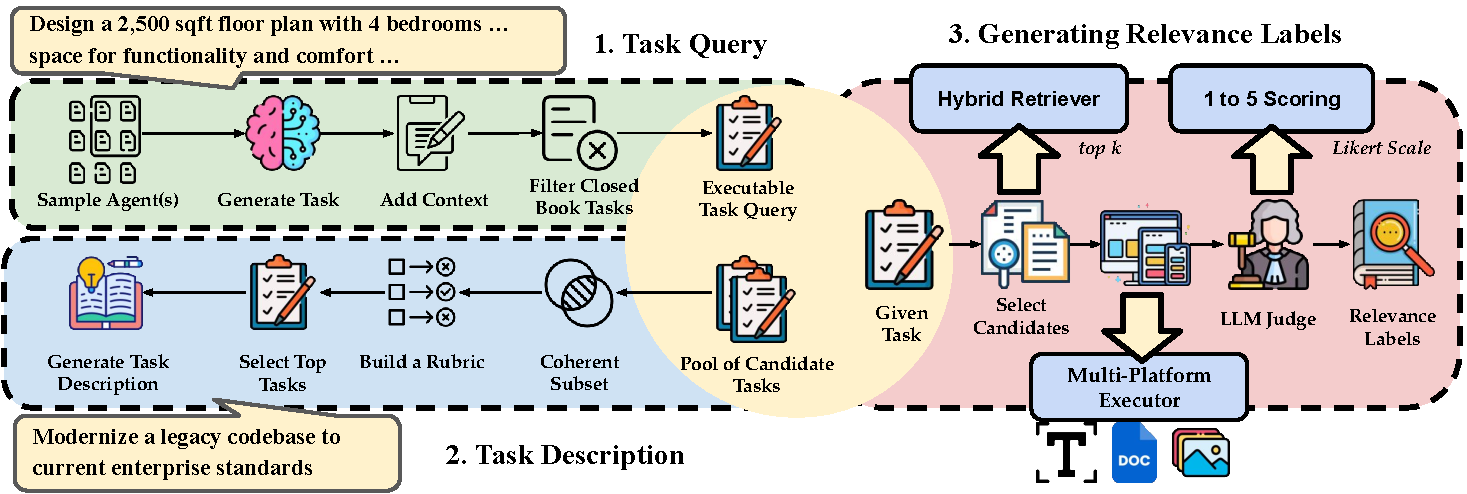
\includegraphics[width=\linewidth]{figures/pipeline.pdf}
\caption{Task and Relevance Label Generation Pipeline of \OURSBENCH{}.}
\label{fig:pipeline}
\end{figure*}

We construct \OURSBENCH{} from a large-scale collection of real-world agents and generate tasks through a hierarchical process. We first create executable task queries, then derive high-level task descriptions grounded in query-level evidence. Relevance is obtained via execution-based evaluation and converted into retrieval and ranking labels. The overall pipeline is shown in \FIG~\ref{fig:pipeline}.

\subsection{Large-Scale Realistic Agent Collection}
We build a repository of nearly 10k agents collected from public platforms, including GPT store\footnote{https://chatgpt.com/gpts}, Google Cloud Marketplace\footnote{https://cloud.google.com/marketplace}, and AgentAI Platform\footnote{https://agent.ai/}. By sourcing agents from real-world ecosystems rather than synthesizing them, AgentBase captures practical challenges such as capability overlap and inconsistent documentation, enabling realistic evaluation of agent search.

\subsection{Task Query Construction}

We synthesize executable task queries from agent documentation following document-grounded task generation \citep{DBLP:conf/iclr/QinLYZYLLCTQZHT24}. To reduce evaluation cost, we retrieve a candidate set of top-$K$ agents using a hybrid scoring function that combines BM25 (lexical) \citep{robertson2009probabilistic}, BGE (semantic) \citep{xiao2024cpack}, and ToolRet (tool-aware) retrieval \citep{shi2025retrieval}:
\begin{align}
s(a,\mathcal{T}_q)=\alpha\,s_{\text{lexical}}+\beta\,s_{\text{semantic}}+\gamma\,s_{\text{tool}}.
\end{align}
Retrieved agents are executed on each query and evaluated using a 5-point LLM-as-judge \citep{gu2024survey}. We filter out degenerate queries where no agent succeeds, or all agents succeed.

Multi-agent queries are constructed by composing executable subtasks from capability-aligned clusters. We retain a composed query only if it semantically entails all subtasks via natural language inference (NLI) \citep{wu2025natural}:
\begin{align}
\mathrm{Entail}(\mathcal{T}_q^{\text{multi}},\mathcal{T}_q^{(i)})=1,\ \forall i.
\end{align}

\subsection{Task Description Construction}

We construct task descriptions by abstracting high-level objectives from clusters of semantically related queries. Given query clusters $\{\mathcal{C}_1,\dots,\mathcal{C}_M\}$, we remove outliers and generate a description $\mathcal{T}_d$ for each cluster using LLMs.

To associate executable queries with each description, we apply a rubric-based judge \citep{sharma2026researchrubrics} that evaluates the relevance of each candidate query $\mathcal{T}_q$ to $\mathcal{T}_d$ from multiple aspects. Formally, let $\mathbf{r}(\mathcal{T}_d,\mathcal{T}_q)=\big(r_1(\mathcal{T}_d,\mathcal{T}_q),\dots,r_D(\mathcal{T}_d,\mathcal{T}_q)\big)$ denote the aspect-wise relevance scores. For each aspect $d$, we select the top-2 queries according to $r_d$, and construct the associated query set as $\mathcal{Q}(\mathcal{T}_d)=\bigcup_{d=1}^{D}\text{Top2}_{\mathcal{T}_q}\, r_d(\mathcal{T}_d,\mathcal{T}_q)$,
resulting in 10 queries when $D=5$. To ensure reliable evaluation, we re-evaluate high-performing agents on missing subtasks and filter inconsistent task descriptions.

\subsection{Relevance Annotation}

Relevance is derived from execution-based performance using a 5-point LLM-as-judge. For retrieval, we convert scores into binary labels:
\begin{align}
\mathrm{rel}(a,\mathcal{T}_q)=\mathbf{1}(y(a,\mathcal{T}_q)\geq 4).
\end{align}

For multi-agent queries and task descriptions, we define graded relevance based on subtask completion:
\begin{align}
r(a,\mathcal{T})=\frac{1}{|\mathcal{S}(\mathcal{T})|}\sum_{\mathcal{T}_q\in\mathcal{S}(\mathcal{T})}\mathrm{rel}(a,\mathcal{T}_q).
\end{align}

To account for documentation–performance misalignment, agents that successfully complete tasks without corresponding documented capability are assigned discounted relevance scores (e.g., 0.5). These signals are used to construct golden rankings for evaluation.

\section{Benchmark Statistic}

\begin{figure*}[t]
\centering

\begin{subfigure}[b]{0.34\textwidth}
\vspace{0pt}
\centering
\small
\resizebox{\linewidth}{!}{%
\begin{tabular}{l r}
\toprule
\multicolumn{2}{l}{\textbf{Statistics}} \\
\midrule
\# Total Agents & 9,759 \\
\# Total Task & 3,211 \\
\quad - \# Single-Agent Task Query & 2,452  \\
\quad - \# Multi-Agent Task Query & 500  \\
\quad - \# Task Description & 259 \\
Avg. query per description & 10 \\
Avg. evaluated agents per query & 20 \\
\# Total executions & 66,740  \\
\bottomrule
\end{tabular}%
}
\caption{Overview statistics.}
\end{subfigure}
\hfill
\begin{subfigure}[b]{0.34\textwidth}
\vspace{0pt}
\centering
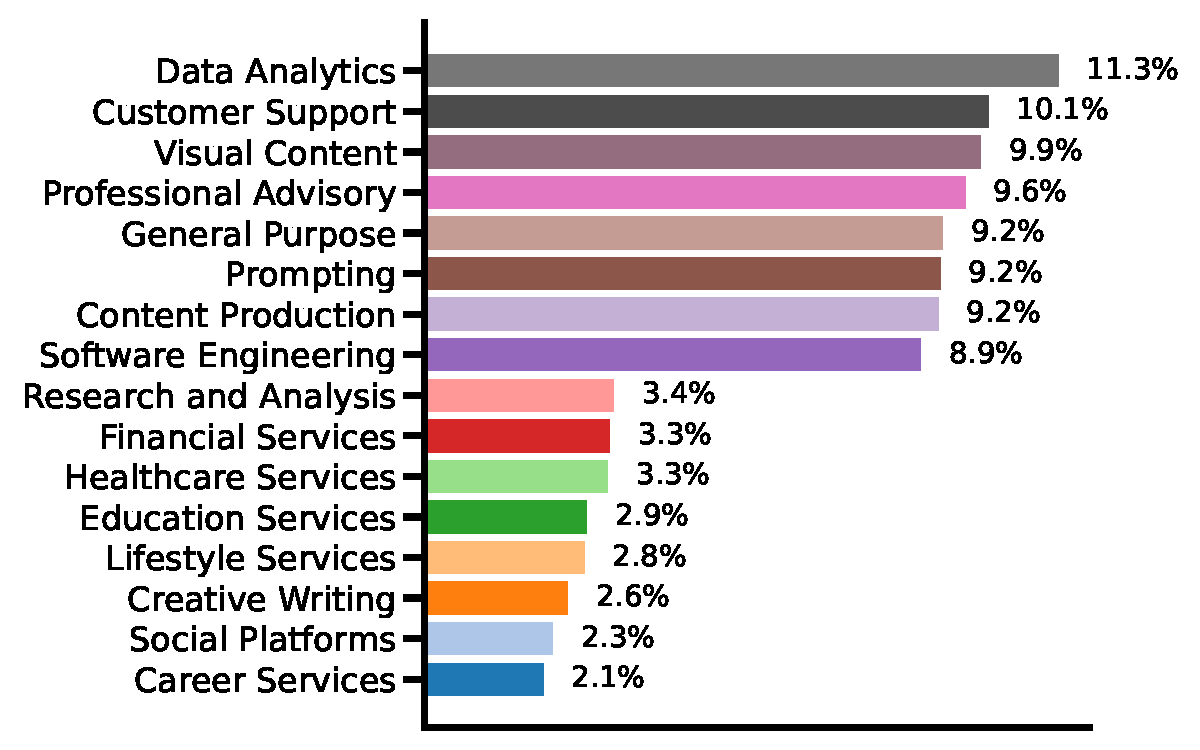
\includegraphics[width=\linewidth]{figures/agent_diversity.pdf}
\caption{Agent diversity.}
\end{subfigure}
\hfill
\begin{subfigure}[b]{0.26\textwidth}
\vspace{0pt}
\centering
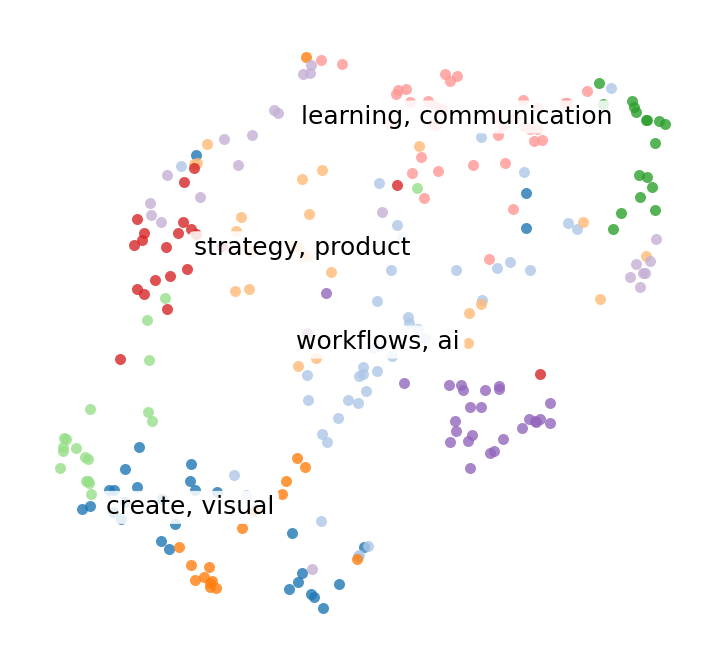
\includegraphics[width=\linewidth]{figures/task_diversity.png}
\caption{Task diversity.}
\end{subfigure}
\vspace{-0.5em}
\caption{Benchmark statistics and semantic diversity of \OURSBENCH{}.}
\vspace{-0.5em}
\label{fig:benchmark_stats}
\end{figure*}

\begin{figure*}[t]
\begin{subfigure}[b]{0.3\textwidth}
\centering
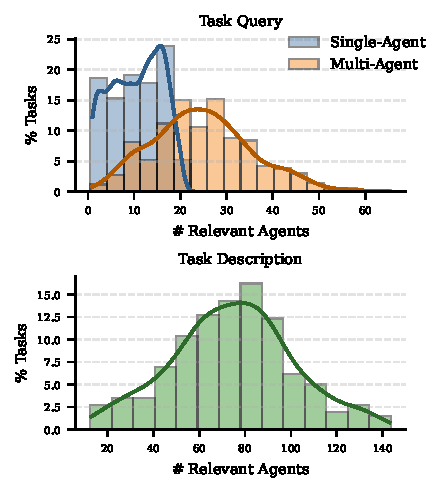
\includegraphics[width=\linewidth]{figures/relevant_agents.pdf}
\caption{Relevant agents per query.}
\end{subfigure}
\hfill
\begin{subfigure}[b]{0.3\textwidth}
\centering
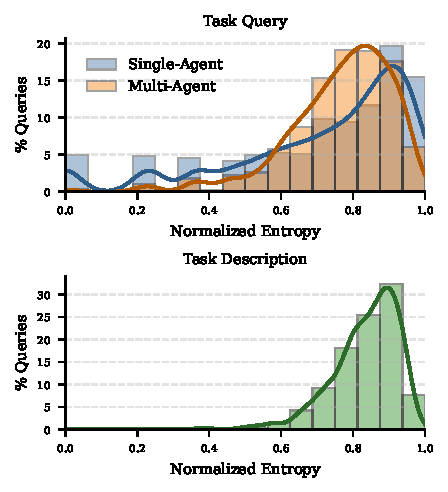
\includegraphics[width=\linewidth]{figures/ranking_label_entropy_distribution.pdf}
\caption{Score entropy.}
\end{subfigure}
\hfill
\begin{subfigure}[b]{0.3\textwidth}
\centering
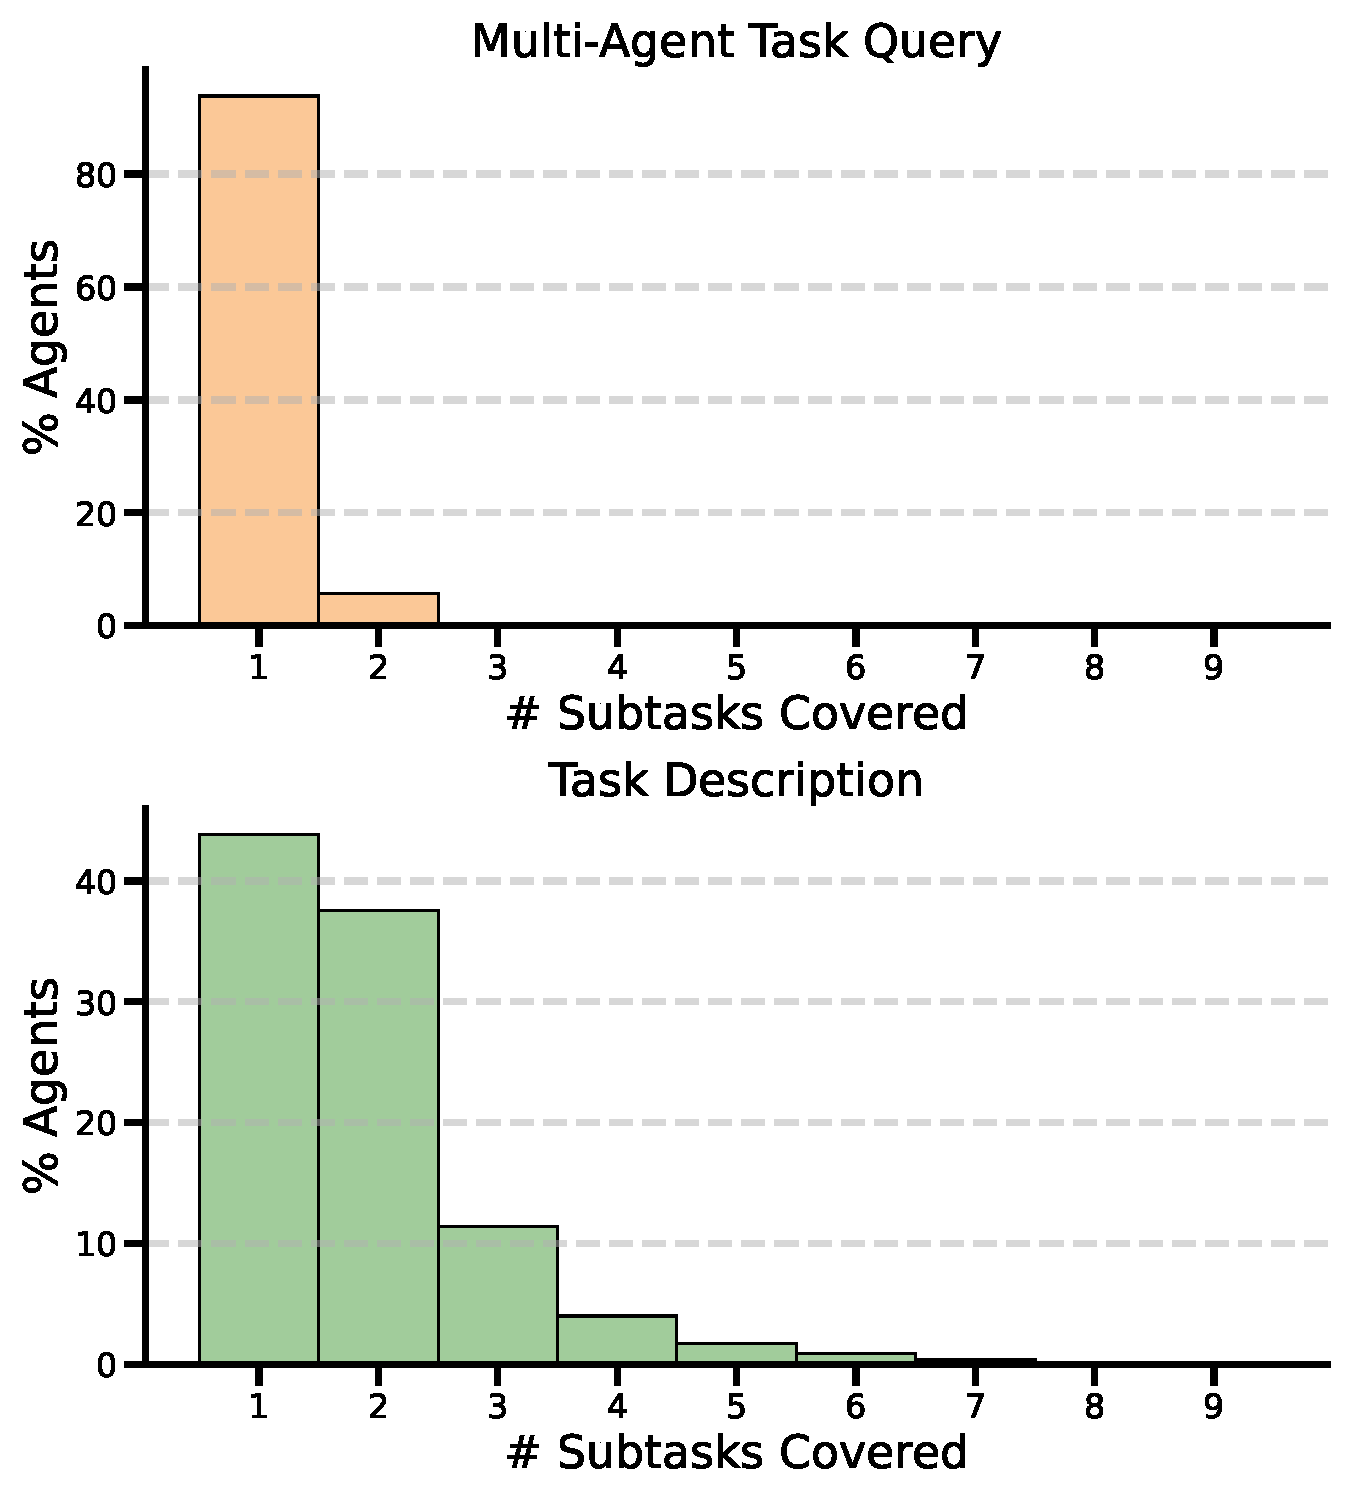
\includegraphics[width=\linewidth]{figures/subtask_coverage.pdf}
\caption{Subtask coverage.}
\end{subfigure}
\vspace{-0.5em}

\caption{Difficulty of Task Query and Task Description of \OURSBENCH{}.}
\vspace{-0.5em}
\label{fig:benchmark_stats_difficulty}
\end{figure*}

We summarize the scale of \OURSBENCH{} in \FIG~\ref{fig:benchmark_stats}. The benchmark contains nearly \textbf{9,760} agents collected from multiple open platforms, among which \textbf{7,867} provide executable interfaces. We construct \textbf{2,952} executable task queries and \textbf{259} task descriptions, each associated with an average of \textbf{10} queries. Each query is evaluated on the top-\textbf{20} retrieved agents, resulting in \textbf{66,740} execution runs. These statistics highlight the scale and execution-centric design of \OURSBENCH{}.

\textbf{Diversity and Difficulty. }
As shown in \FIG~\ref{fig:benchmark_stats}(b–c), both agents and tasks exhibit broad and long-tailed semantic distributions, reflecting diverse capability coverage. \FIG~\ref{fig:benchmark_stats_difficulty}(a) shows that many queries have multiple relevant agents, making retrieval alone insufficient. Meanwhile, the entropy distribution in \FIG~\ref{fig:benchmark_stats_difficulty}(b) indicates substantial performance variance across agents, motivating fine-grained reranking. Finally, \FIG~\ref{fig:benchmark_stats_difficulty}(c) shows that agents typically cover only a subset of subtasks, highlighting partial and overlapping capabilities. Overall, \OURSBENCH{} provides a realistic and challenging setting for performance-grounded agent search.

\section{Agent Search Evaluation}


\begin{table}[!t]
\centering
\renewcommand{\arraystretch}{1.25}
\resizebox{\textwidth}{!}{%
\begin{tabular}{lccccccccccccc}
\toprule
\textbf{Model} & \textbf{Type} & \multicolumn{3}{c}{\textbf{NDCG}} & \multicolumn{3}{c}{\textbf{Precision}} & \multicolumn{3}{c}{\textbf{Recall}} & \multicolumn{3}{c}{\textbf{Completeness}}\\
\cline{3-14}
 & & \textbf{@5} & \textbf{@10} & \textbf{@20} & \textbf{@5} & \textbf{@10} & \textbf{@20} & \textbf{@5} & \textbf{@10} & \textbf{@20} & \textbf{@5} & \textbf{@10} & \textbf{@20} \\
\midrule
\rowcolor{lavenderblush}\multicolumn{14}{c}{\textit{Task Query}} \\
\hline
SPLADE v2 & Sparse & 4.09 & 3.49 & 3.48 & 4.09 & 3.19 & 2.29 & 0.35 & 1.35 & 3.72 & 2.90 & 9.21 & 18.93 \\
BM25 & Sparse & \cellcolor{aliceblue}\textbf{32.41} & \cellcolor{aliceblue}\textbf{26.73} & \cellcolor{aliceblue}\textbf{22.68} & \cellcolor{aliceblue}\textbf{32.41} & \cellcolor{aliceblue}\textbf{24.56} & \cellcolor{aliceblue}\textbf{14.07} & \cellcolor{aliceblue}\textbf{2.62} & \cellcolor{aliceblue}\textbf{9.33} & \cellcolor{aliceblue}\textbf{21.36} & \cellcolor{aliceblue}\textbf{20.81} & \cellcolor{aliceblue}\textbf{38.10} & \cellcolor{aliceblue}\textbf{51.38} \\
\hline
ColBERT v2 & Dense & 27.71 & 23.07 & 20.47 & 27.71 & 21.14 & 13.44 & 2.12 & 7.94 & 19.68 & 16.52 & 33.89 & 43.95 \\
Contriever MS-Marco & Dense & 20.75 & 17.43 & 16.72 & 20.75 & 16.11 & 11.12 & 1.72 & 6.34 & 17.07 & 15.04 & 30.73 & 45.11 \\
GTR-T5 Base & Dense & 23.20 & 19.50 & 17.55 & 23.20 & 18.05 & 11.51 & 1.89 & 6.87 & 16.92 & 16.00 & 32.09 & 44.63 \\
MiniLM-L6 v2 & Dense & 29.02 & 25.28 & 22.46 & 29.02 & 23.57 & 14.97 & 2.29 & 8.63 & 21.33 & 18.23 & 36.52 & 51.52 \\
BGE-Large v1.5 & Dense & \cellcolor{aliceblue}\textbf{31.78} & \cellcolor{aliceblue}\textbf{28.24} & \cellcolor{aliceblue}\textbf{26.14} & \cellcolor{aliceblue}\textbf{31.78} & \cellcolor{aliceblue}\textbf{26.48} & \cellcolor{aliceblue}\textbf{17.64} & \cellcolor{aliceblue}\textbf{2.48} & \cellcolor{aliceblue}\textbf{10.07} & \cellcolor{aliceblue}\textbf{25.49} & \cellcolor{aliceblue}\textbf{20.18} & \cellcolor{aliceblue}\textbf{38.61} & \cellcolor{aliceblue}\textbf{52.52} \\
\hline
COLT ToolLens & Tool & 9.35 & 8.12 & 7.91 & 9.35 & 7.59 & 5.47 & 0.81 & 2.92 & 7.85 & 6.95 & 18.07 & 30.61 \\
COLT ToolBench & Tool & 16.25 & 13.84 & 12.28 & 16.25 & 12.81 & 8.00 & 1.30 & 4.82 & 12.13 & 11.74 & 25.39 & 38.66 \\
Tool-Embed & Tool & 34.02 & 28.40 & 25.67 & 34.02 & 26.37 & 17.23 & 2.50 & 9.77 & 24.46 & 20.22 & 38.14 & 53.91 \\
ToolRet & Tool & \cellcolor{aliceblue}\textbf{37.52} & \cellcolor{aliceblue}\textbf{31.73} & \cellcolor{aliceblue}\textbf{28.87} & \cellcolor{aliceblue}\textbf{37.52} & \cellcolor{aliceblue}\textbf{29.36} & \cellcolor{aliceblue}\textbf{19.36} & \cellcolor{aliceblue}\textbf{2.85} & \cellcolor{aliceblue}\textbf{10.97} & \cellcolor{aliceblue}\textbf{27.80} & \cellcolor{aliceblue}\textbf{21.91} & \cellcolor{aliceblue}\textbf{42.18} & \cellcolor{aliceblue}\textbf{57.53} \\
\hline
E5-Mistral 7B & Decoder-only & 19.57 & 16.31 & 15.29 & 19.57 & 14.99 & 9.77 & 1.60 & 6.05 & 15.62 & 15.27 & 30.71 & 44.49 \\
Qwen-Embedding 8B & Decoder-only & \cellcolor{aliceblue}\textbf{25.25} & \cellcolor{aliceblue}\textbf{22.59} & \cellcolor{aliceblue}\textbf{21.43} & \cellcolor{aliceblue}\textbf{25.25} & \cellcolor{aliceblue}\textbf{21.32} & \cellcolor{aliceblue}\textbf{14.83} & \cellcolor{aliceblue}\textbf{1.94} & \cellcolor{aliceblue}\textbf{7.81} & \cellcolor{aliceblue}\textbf{21.14} & \cellcolor{aliceblue}\textbf{16.15} & \cellcolor{aliceblue}\textbf{33.17} & \cellcolor{aliceblue}\textbf{48.33} \\
\midrule
\rowcolor{oldlace}\multicolumn{14}{c}{\textit{Task Description}} \\
\hline
SPLADE v2 & Sparse & 12.02 & 8.24 & 6.93 & 12.02 & 7.50 & 6.11 & 0.35 & 0.83 & 2.49 & 0.00 & 0.00 & \cellcolor{aliceblue}\textbf{0.48} \\
BM25 & Sparse & \cellcolor{aliceblue}\textbf{16.35} & \cellcolor{aliceblue}\textbf{13.42} & \cellcolor{aliceblue}\textbf{10.78} & \cellcolor{aliceblue}\textbf{16.35} & \cellcolor{aliceblue}\textbf{12.50} & \cellcolor{aliceblue}\textbf{9.25} & \cellcolor{aliceblue}\textbf{0.46} & \cellcolor{aliceblue}\textbf{1.28} & \cellcolor{aliceblue}\textbf{3.69} & 0.00 & 0.00 & \cellcolor{aliceblue}\textbf{0.48} \\
\hline
ColBERT v2 & Dense & 15.38 & 13.19 & 12.80 & 15.38 & 12.31 & 12.19 & 0.27 & 1.14 & 5.12 & 0.00 & 0.48 & 1.92 \\
Contriever MS-Marco & Dense & 15.38 & 15.03 & 14.22 & 15.38 & 14.81 & 13.37 & 0.31 & 1.49 & 5.70 & 0.00 & 0.48 & 1.92 \\
GTR-T5 Base & Dense & 15.87 & 15.03 & 12.96 & 15.87 & 14.52 & 11.92 & 0.34 & 1.56 & 4.93 & 0.00 & 0.00 & 1.92 \\
MiniLM-L6 v2 & Dense & 20.67 & 17.69 & 15.84 & 20.67 & 17.02 & \cellcolor{aliceblue}\textbf{14.57} & \cellcolor{aliceblue}\textbf{0.59} & 1.84 & \cellcolor{aliceblue}\textbf{6.24} & 0.00 & 0.48 & 1.44 \\
BGE-Large v1.5 & Dense & \cellcolor{aliceblue}\textbf{23.08} & \cellcolor{aliceblue}\textbf{19.26} & \cellcolor{aliceblue}\textbf{16.07} & \cellcolor{aliceblue}\textbf{23.08} & \cellcolor{aliceblue}\textbf{18.08} & 14.40 & 0.42 & \cellcolor{aliceblue}\textbf{1.94} & 6.12 & 0.00 & \cellcolor{aliceblue}\textbf{0.96} & \cellcolor{aliceblue}\textbf{3.37} \\
\hline
COLT ToolLens & Tool & 11.06 & 10.11 & 8.60 & 11.06 & 9.90 & 7.88 & 0.18 & 1.05 & 3.47 & 0.00 & 0.00 & 0.96 \\
COLT ToolBench & Tool & 12.50 & 12.64 & 11.57 & 12.50 & 12.60 & 10.84 & 0.28 & 1.49 & 4.53 & 0.00 & 0.48 & 1.92 \\
Tool-Embed & Tool & \cellcolor{aliceblue}\textbf{21.15} & \cellcolor{aliceblue}\textbf{20.08} & 17.19 & \cellcolor{aliceblue}\textbf{21.15} & \cellcolor{aliceblue}\textbf{19.81} & \cellcolor{aliceblue}\textbf{15.94} & \cellcolor{aliceblue}\textbf{0.42} & 2.01 & 6.41 & 0.00 & 0.48 & 1.92 \\
ToolRet & Tool & \cellcolor{aliceblue}\textbf{21.15} & 19.87 & \cellcolor{aliceblue}\textbf{17.21} & \cellcolor{aliceblue}\textbf{21.15} & 19.13 & 15.77 & 0.37 & \cellcolor{aliceblue}\textbf{2.02} & \cellcolor{aliceblue}\textbf{6.69} & 0.00 & \cellcolor{aliceblue}\textbf{0.96} & \cellcolor{aliceblue}\textbf{3.37} \\
\hline
E5-Mistral 7B & Decoder-only & 15.87 & 14.78 & 11.56 & 15.87 & 14.71 & 10.22 & 0.33 & 1.74 & 4.58 & 0.00 & \cellcolor{aliceblue}\textbf{0.48} & 1.92 \\
Qwen-Embedding 8B & Decoder-only & \cellcolor{aliceblue}\textbf{20.67} & \cellcolor{aliceblue}\textbf{18.84} & \cellcolor{aliceblue}\textbf{16.51} & \cellcolor{aliceblue}\textbf{20.67} & \cellcolor{aliceblue}\textbf{18.08} & \cellcolor{aliceblue}\textbf{15.29} & \cellcolor{aliceblue}\textbf{0.46} & \cellcolor{aliceblue}\textbf{1.87} & \cellcolor{aliceblue}\textbf{6.15} & 0.00 & 0.00 & \cellcolor{aliceblue}\textbf{2.40} \\
\bottomrule
\end{tabular}%
}
\caption{Retrieval results on Task Query $T_q$ (Single-Agent and Multi-Agent Task Queries) and Task Descriptions $T_d$. We \colorbox{aliceblue}{\textbf{highlight}} the best performance in each type of model.}
\label{tab:retrieval}
\end{table}

\begin{table}[!t]
\centering
\renewcommand{\arraystretch}{1.25}
\resizebox{\textwidth}{!}{%
\begin{tabular}{lccccccccccc}
\toprule
\textbf{Model} & \textbf{Type} & \multicolumn{3}{c}{\textbf{NDCG}} & \multicolumn{2}{c}{\textbf{Completeness}} & \multicolumn{3}{c}{\textbf{NDCG}} & \multicolumn{2}{c}{\textbf{Completeness}}\\
\cline{3-12}
 & & \textbf{@1} & \textbf{@5} & \textbf{@20} & \textbf{@1} & \textbf{@5} &\textbf{@1} & \textbf{@5} & \textbf{@20} & \textbf{@1} & \textbf{@5 } \\
\midrule
&&\multicolumn{5}{c}{\cellcolor{lavenderblush}\textit{Task Query}} &\multicolumn{5}{c}{\cellcolor{oldlace}\textit{Task Description}} \\
\hline
Random Shuffle & / & 51.43 & 50.98 & 74.61 & 28.50 & 61.00 & 53.00 & 48.27 & 76.60 & 0.00 & 0.00 \\
\hline
MiniLM-L12 v2 & Cross-Encoder & 48.27 & 48.06 & 73.53 & 28.50 & 52.00 & 48.00 & 57.49 & 81.58 & 0.00 & 0.00 \\
MXBAI Reranker Large & Cross-Encoder & 52.09 & 53.42 & 76.32 & 30.00 & 58.00 & 52.84 & \cellcolor{aliceblue}\textbf{61.33} & \cellcolor{aliceblue}\textbf{82.22} & 0.00 & 0.48 \\
BGE Reranker v2 & Cross-Encoder & \cellcolor{aliceblue}\textbf{63.09} & \cellcolor{aliceblue}\textbf{59.84} & \cellcolor{aliceblue}\textbf{79.59} & \cellcolor{aliceblue}\textbf{30.50} & \cellcolor{aliceblue}\textbf{59.00} & \cellcolor{aliceblue}\textbf{54.31} & 60.55 & 81.97 & 0.00 & \cellcolor{aliceblue}\textbf{0.96} \\
\hline
Tool-Rank 4B & Tool & 63.84 & \cellcolor{aliceblue}\textbf{64.45} & 81.78 & 28.00 & 59.50 & 52.24 & 61.12 & 82.32 & 0.00 & 0.48 \\
Tool-Rank 8B & Tool & \cellcolor{aliceblue}\textbf{66.67} & 64.36 & \cellcolor{aliceblue}\textbf{81.96} & \cellcolor{aliceblue}\textbf{30.50} & \cellcolor{aliceblue}\textbf{60.00} & \cellcolor{aliceblue}\textbf{53.92} & \cellcolor{aliceblue}\textbf{61.97} & \cellcolor{aliceblue}\textbf{82.76} & 0.00 & \cellcolor{aliceblue}\textbf{0.96} \\
\hline
MonoT5 Base MS-Marco & Decoder-only  & 57.84 & 57.37 & 78.69 & 27.00 & 60.00 & 52.31 & 59.10 & 81.33 & 0.00 & 0.96  \\
Qwen Reranker 0.6B & Decoder-only & 63.34 & 63.72 & 81.08 & \cellcolor{aliceblue}\textbf{30.50} & 58.50 & 53.96 & 60.47 & 82.04 & 0.00 & 0.48 \\
Qwen Reranker 4B & Decoder-only & \cellcolor{aliceblue}\textbf{64.67} & \cellcolor{aliceblue}\textbf{64.53} & \cellcolor{aliceblue}\textbf{81.97} & 29.50 & \cellcolor{aliceblue}\textbf{62.50} & \cellcolor{aliceblue}\textbf{58.00} & \cellcolor{aliceblue}\textbf{60.58} & \cellcolor{aliceblue}\textbf{82.84} & 0.00 & 0.00 \\
\hline
RankGPT Qwen-3 32B & LLM-based & 61.00 & 61.05 & 80.18 & 29.00 & \cellcolor{aliceblue}\textbf{58.50} & 53.95 & 60.78 & 82.36 & 0.00 & 0.48 \\
RankGPT LLaMA-3.3 70B & LLM-based & 61.09 & 59.92 & 79.80 & 29.50 & 53.50 & 52.60 & 61.24 & 82.34 & 0.00 & \cellcolor{aliceblue}\textbf{0.96} \\
RankGPT GPT-5.2 & LLM-based & \cellcolor{aliceblue}\textbf{63.59} & \cellcolor{aliceblue}\textbf{64.57} & \cellcolor{aliceblue}\textbf{81.88} & \cellcolor{aliceblue}\textbf{30.50} & 56.50 & \cellcolor{aliceblue}\textbf{66.00} & \cellcolor{aliceblue}\textbf{64.66} & \cellcolor{aliceblue}\textbf{84.69} & 0.00 & 0.00 \\
\bottomrule
\end{tabular}%
}
\caption{Reranking results on Task Query $T_q$ (Single-Agent and Multi-Agent Task Queries) and Task Descriptions $T_d$. We \colorbox{aliceblue}{\textbf{highlight}} the best performance in each type of model.}
\vspace{-0.5em}
\label{tab:rerank}
\end{table}






\subsection{Experimental Setup}

We evaluate agent search under both executable task queries and high-level task descriptions. For retrieval, methods search over the full agent repository using binary relevance labels derived from execution outcomes. For reranking, each method is given the top-20 agents with highest execution-based relevance and is evaluated against the golden ranking induced by aggregated subtask completion performance.

For retrieval, we report Precision, Recall, NDCG, and Completeness \citep{qu2024towards, shi2025retrieval}. For reranking, we report NDCG and Completeness using graded relevance labels. We compare representative methods from four retrieval families, including sparse, dense, tool-aware, and decoder-only embedding models \citep{robertson2009probabilistic, formal2021splade, santhanam2022colbertv2, izacard2021unsupervised, ni2022large, wang2021minilmv2, xiao2024cpack, shi2025retrieval, lu2025tools, qu2024towards}, and four reranking families, including cross-encoders, tool-specific rankers, decoder-only rerankers, and LLM-based rankers \citep{wang2021minilmv2, multi2024m3, li2025prorank, lu2025tools, nogueira2020document, qwen3embedding, sun2023chatgpt, ma2024fine}. All methods retrieve or rerank a fixed top-$K$ candidate set under the same evaluation protocol.

\subsection{Benchmarking Analysis}

\TAB~\ref{tab:retrieval} shows retrieval performance under execution-based relevance. On task queries, tool-aware retrievers outperform dense and sparse baselines, while on task descriptions, dense retrievers become more competitive, with BGE achieving the strongest overall performance. However, performance drops substantially when moving from executable queries to high-level task descriptions, and completeness remains low across all methods, highlighting the difficulty of retrieving agents that can fully satisfy abstract requirements. \textbf{Overall, these results indicate that while retrieval can capture coarse relevance, it struggles to identify agents with comprehensive task-solving capability, especially under high-level task specifications without explicit executable demands.}

\TAB~\ref{tab:rerank} shows reranking results on execution-grounded candidate pools. On task queries, different model families achieve broadly similar performance, suggesting that surface-level signals are often sufficient for relatively concrete tasks. On task descriptions, however, \textbf{decoder-only and LLM-based rerankers perform more strongly, possibly because their stronger generative capacity helps infer latent or implicit requirements behind high-level task descriptions.} Nevertheless, completeness remains limited, showing that improved ordering does not fully resolve the challenge of identifying agents that can completely satisfy complex requirements.

To further examine this limitation, \FIG~\ref{fig:surface-gap} compares accumulated golden performance under model rankings with the oracle ranking. All methods remain substantially below the oracle, with gains distributed gradually rather than concentrated at top ranks. This indicates that many high-performing agents are ranked too low, reflecting \textbf{a misalignment between agent documentation and actual execution performance}. This misalignment leads to a persistent semantic–performance gap, where documentation-based matching fails to accurately capture execution effectiveness.

\begin{figure*}[t]
\centering
\begin{subfigure}[b]{0.30\textwidth}
\vspace{0pt}
\centering
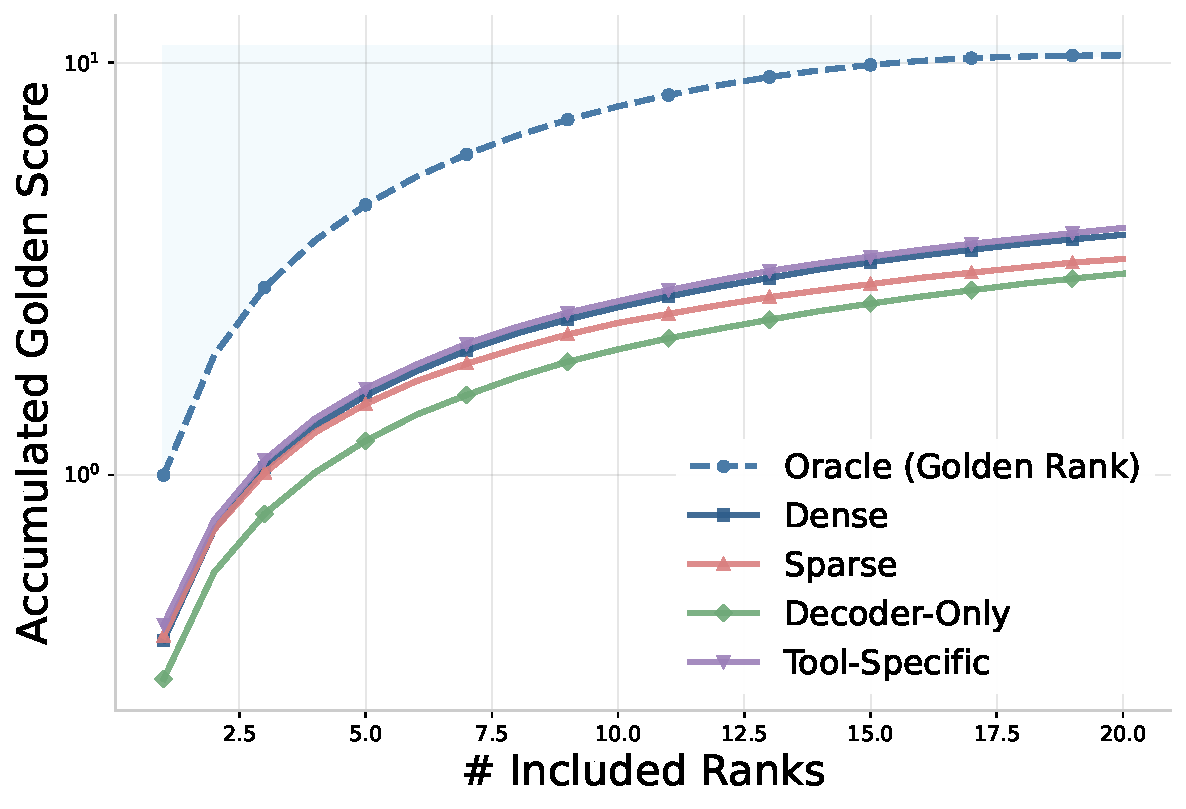
\includegraphics[width=\linewidth]{figures/agent_semantic_per_single_tq.pdf}
\caption{Golden ranking accumulated agent scores on 2452 Single-Agent Task Queries. }
\label{fig:semantic-gap-single}
\end{subfigure}
\hfill
\begin{subfigure}[b]{0.30\textwidth}
\vspace{0pt}
\centering
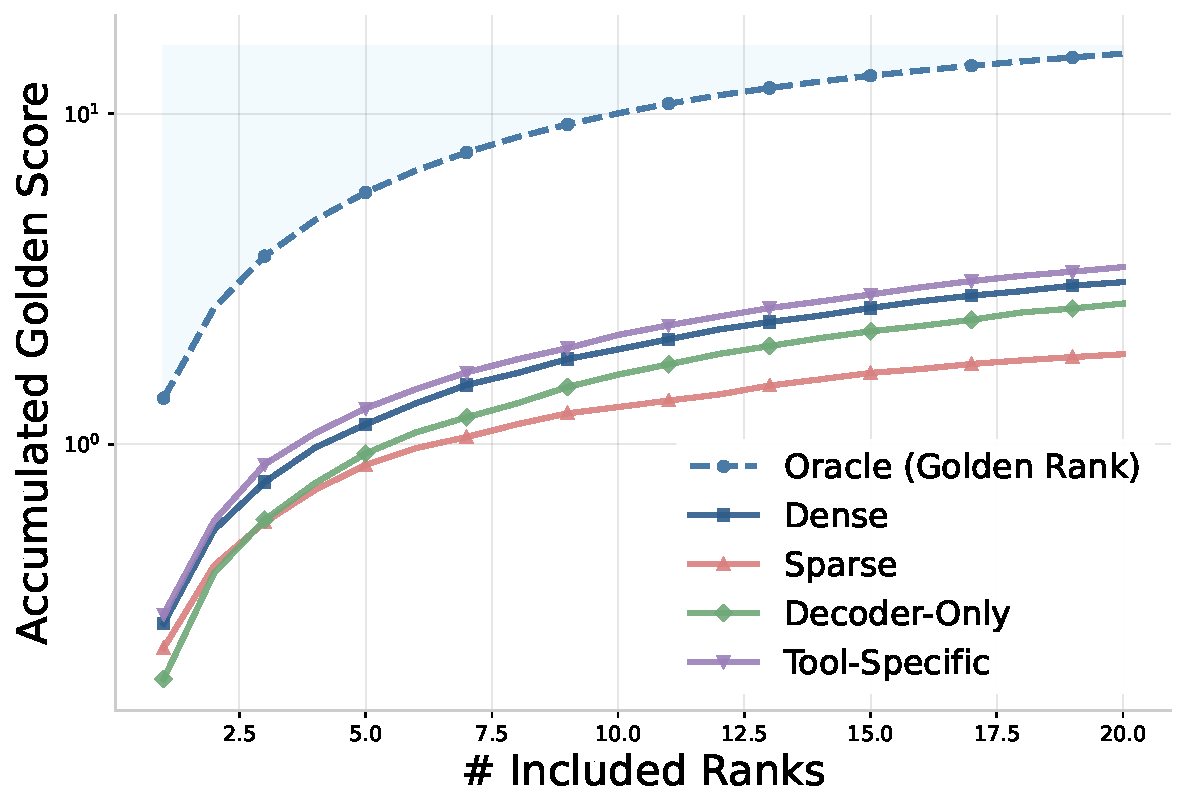
\includegraphics[width=\linewidth]{figures/agent_semantic_per_multi_tq.pdf}\caption{Golden ranking accumulated agent scores on 500 Multi-Agent Task Queries.}
\label{fig:semantic-gap-multi}
\end{subfigure}
\hfill
\begin{subfigure}[b]{0.30\textwidth}
\vspace{0pt}
\centering
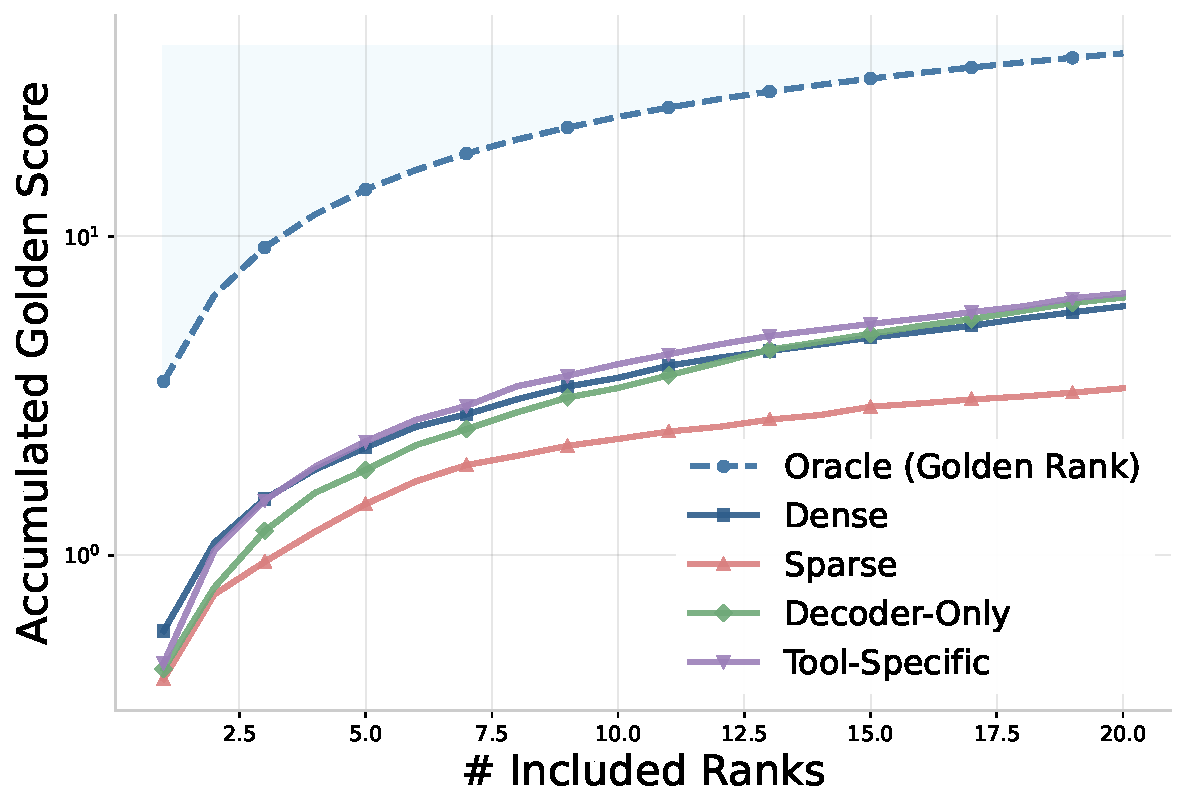
\includegraphics[width=\linewidth]{figures/agent_semantic_per_td.pdf}
\caption{Golden ranking accumulated agent scores on 259 Task Descriptions.}
\label{fig:semantic-gap-td}
\end{subfigure}
\caption{The Gap between Surface-matching and Execution.}
\label{fig:surface-gap}
\end{figure*}


\subsection{Benchmark Validation}

We validate the realism of our benchmark by comparing retrieval trends on synthetic queries with those on external realistic benchmarks. As shown in Figure~\ref{fig:synthetic_realistic}, representative sparse, dense, and tool-aware retrievers exhibit consistent relative trends across settings: dense and tool-aware methods remain substantially stronger than sparse retrieval, while absolute performance on realistic queries is notably lower. \textbf{This suggests that our synthetic benchmark preserves the relative performance ordering of different methods while providing a controlled evaluation setting.} In contrast, realistic queries are inherently more difficult, as they do not guarantee the existence of highly relevant agents in the candidate pool, resulting in lower absolute performance.

We further validate the reliability of LLM-based relevance annotation by comparing it with human judgments. Following the relevance label in our \OURSBENCH{}, we focus on binary relevance signals by grouping scores of 4–5 as positive and 1–3 as negative, which are the primary signals used in our benchmark. We conduct a human evaluation on 500 execution instances with three AI PhD-level annotators and observe high agreement between LLM-based and human judgments, with a Cohen's kappa of $\kappa=0.93$ and accuracy $96.67\%$. \textbf{These results indicate that LLM-as-judge provides reliable supervision for large-scale evaluation, supporting its use for constructing execution-grounded relevance labels.}

\begin{figure*}[t]
\centering

\begin{subfigure}[b]{0.36\textwidth}
\vspace{0pt}
\centering
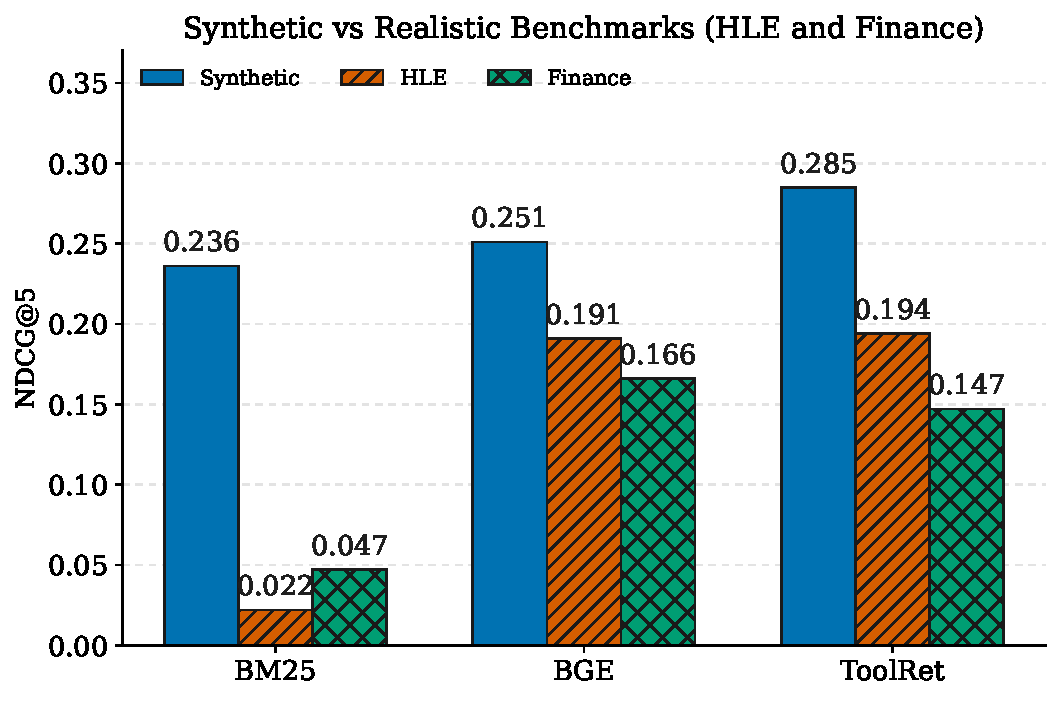
\includegraphics[width=\linewidth]{figures/synthetic_vs_realistic.pdf}
\caption{NDCG@5: Comparison between Realistic and Synthetic Single-agent Task Queries.}
\label{fig:synthetic_realistic}
\end{subfigure}
\hfill
\begin{subfigure}[b]{0.3\textwidth}
\vspace{0pt}
\centering
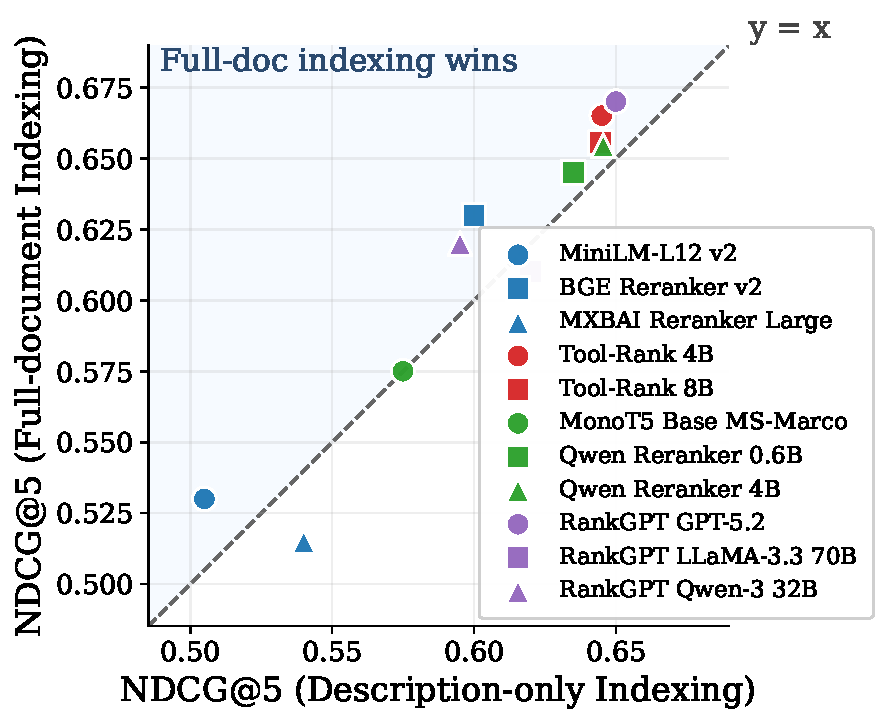
\includegraphics[width=\linewidth]{figures/indexing_task_query.pdf}
\caption{NDCG@5: description-only vs full-document indexing on 2,952 Task Queries.}
\label{fig:indexing_retrieval}
\end{subfigure}
\hfill
\begin{subfigure}[b]{0.3\textwidth}
\vspace{0pt}
\centering
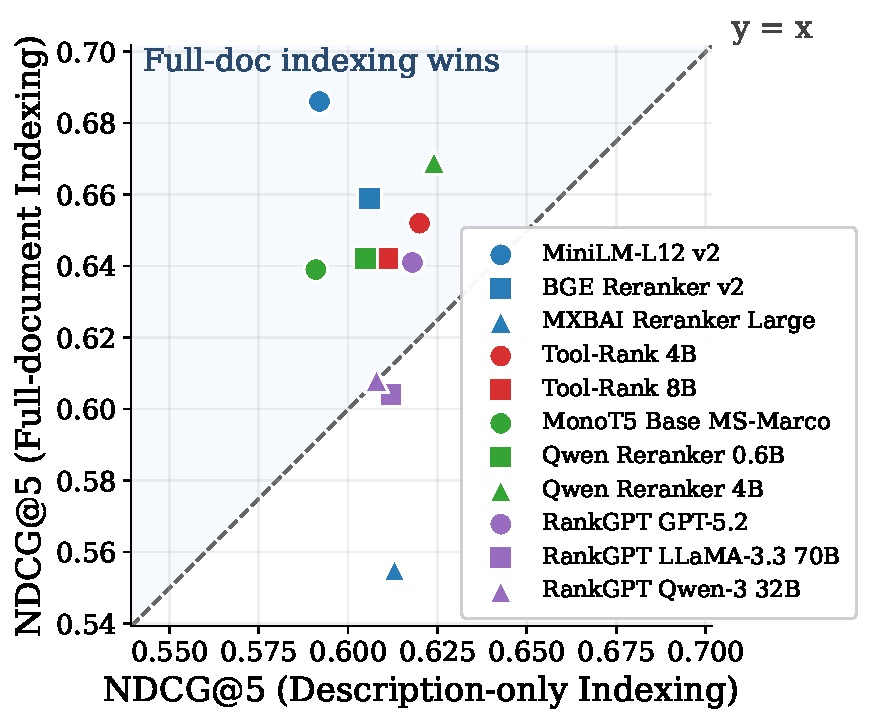
\includegraphics[width=\linewidth]{figures/indexing_task_desc.pdf}
\caption{NDCG@5: description-only vs full-document indexing on 259 Task Descriptions.}
\label{fig:indexing_reranking}
\end{subfigure}

\caption{
Comparison between indexing and query realism.}
\label{fig:rq6_rq4_analysis}
\end{figure*}

\subsection{Execution-Aware Probing}

We next study whether lightweight behavioral signals can improve agent ranking. First, we compare description-only indexing with full-document indexing that additionally includes usage examples. As shown in \FIG~\ref{fig:indexing_retrieval} and \FIG~\ref{fig:indexing_reranking}, most methods improve under full-document indexing. \textbf{These observations suggest that usage examples, often provided and verified by developers through execution, offer behavioral evidence beyond static descriptions.}

We then investigate explicit probing, where LLMs generate probing queries, candidate agents are executed on these queries, and the resulting responses are used as additional ranking signals. \FIG~\ref{fig:winrate} shows that probing is most effective when the probing responses exhibit medium or high variance across agents, whereas low-variance probes provide limited discrimination. Using these execution-derived signals, most rerankers achieve consistent improvements as shown in \FIG~\ref{tab:rerank_probing}, demonstrating that \textbf{lightweight behavioral probing can complement description-based ranking and better capture execution-level capability}.

\begin{figure*}[t]
\centering
\begin{subfigure}[b]{0.5\textwidth}
\vspace{0pt}
\centering
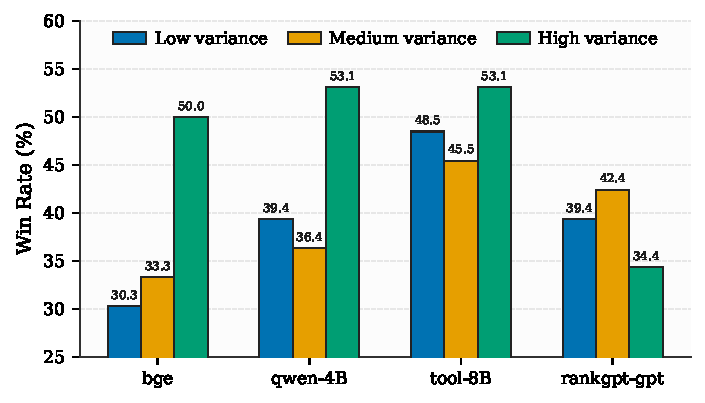
\includegraphics[width=\textwidth]{figures/winrate_by_variance_groups.pdf}
\caption{NDCG@5: win rate v.s. probe score variance}
\label{fig:winrate}
\end{subfigure}
\hspace{1em}
\begin{subfigure}[b]{0.4\textwidth}
\vspace{0pt}
\centering
\renewcommand{\arraystretch}{1.25}
\resizebox{\textwidth}{!}{%
\begin{tabular}{lll}
\toprule
\textbf{Model} & {\textbf{NDCG@5}} & {\textbf{NDCG@10}}\\
\midrule
BGE Reranker v2            & 57.93              & 80.76              \\
\quad w/ Probing           & 58.16~\up{+0.40\%} & 80.82~\up{+0.07\%} \\
\hline
Tool-Rank 8B               & 60.82              & 82.09              \\
\quad w/ Probing           & 61.71~\up{+1.46\%} & 82.24~\up{+0.18\%} \\
\hline
Qwen Reranker 4B           & 60.96              & 82.12              \\
\quad w/ Probing           & 61.91~\up{+1.56\%} & 82.38~\up{+0.32\%} \\
\hline
RankGPT GPT-5.2            & 61.25              & 82.40              \\
\quad w/ Probing           & 59.60~\dn{-2.69\%} & 82.94~\up{+0.66\%} \\
\bottomrule
\end{tabular}
}
\caption{Execution-Aware Probing enhancements on 100 Task Descriptions $T_d$.}
\label{tab:rerank_probing}
\end{subfigure}
\caption{Execution-Aware Probing for Reranking on Task Description.}
\vspace{-1em}
\label{fig:probing}
\end{figure*}




\section{Conclusion}

We introduce \OURSBENCH{}, a large-scale benchmark for agent search in open ecosystems, covering nearly 10,000 real-world agents and supporting both executable task queries and high-level task descriptions. By grounding relevance in execution outcomes, our benchmark reveals a substantial semantic–performance gap: methods based on textual similarity often fail to identify the best-performing agents. While existing retrieval and reranking approaches provide useful coarse signals, they remain limited in capturing execution-dependent capability, especially for abstract and multi-step tasks. We show that incorporating lightweight behavioral signals, such as richer indexing and execution-aware probing, can improve ranking quality. These results highlight the importance of execution-aware methods and establish \OURSBENCH{} as a practical testbed for performance-grounded agent search.

% \section*{Author Contributions}
% If you'd like to, you may include a section for author contributions as is done
% in many journals. This is optional and at the discretion of the authors.

% \section*{Acknowledgments}
% Use unnumbered first level headings for the acknowledgments. All
% acknowledgments, including those to funding agencies, go at the end of the paper.

% \section*{Ethics Statement}
% Authors can add an optional ethics statement to the paper. 
% For papers that touch on ethical issues, this section will be evaluated as part of the review process. The ethics statement should come at the end of the paper. It does not count toward the page limit, but should not be more than 1 page. 


\bibliography{main}
\bibliographystyle{colm2026_conference}

\clearpage
\appendix
\section{More Details about \OURSBENCH{}}

\subsection{Schema Design}

A key challenge in constructing AgentBase lies in the heterogeneous representation of agents across platforms, where capability descriptions, usage instructions, and accessibility conditions are presented in inconsistent formats. To enable systematic indexing and fair comparison in agent search, we introduce a unified schema that standardizes agent information into four semantic groups:
(1) \textit{Agent metadata} provides stable identity and provenance signals, supporting deduplication and version tracking;
(2) \textit{Capability description} captures the functional semantics of agents through textual descriptions, category tags, and modality indicators;
(3) \textit{Usage guidance} characterizes how agents are invoked and interacted with in practice, including quick-start instructions and example interactions;
(4) \textit{Availability and constraints} record practical deployment conditions such as pricing, accessibility, base models, and update timestamps, reflecting real-world feasibility considerations.
This structured representation enables scalable agent collection, consistent retrieval over heterogeneous sources, and reproducible evaluation of agent search systems.
We show our schema design in \TAB~\ref{tab:schema} and one example in \TAB~\ref{tab:schema-example}.

\subsection{Example of Task Query and Task Description}

We show the example of single-and multi-agent task query, and task description in \TAB~\ref{tab:task-example}.

\subsection{Implementation Details of Benchmark Construction}

We use GPT-5.2 as the backbone for all generation steps with temperature $\tau = 1$. For task description generation, we begin with a candidate pool of 100 task queries, which are filtered down to 10 via rubric-based scoring across 5 criteria, each criterion associated with approximately 2 subtasks. For multi-agent task query we pick 2–4 subtasks (mean 2.91), sampled to be semantically related yet non-redundant. Concretely, given an anchor task query, we retrieve the top-$K$ most similar candidates and skip the highest-ranked $k_{\text{skip}}$ to avoid near-duplicate subtasks.

We retrieve a candidate set of top-$K$ agents using a hybrid scoring function
combining BM25~\citep{robertson2009probabilistic}, BGE~\citep{xiao2024cpack},
and ToolRet~\citep{shi2025retrieval} as lexical, semantic, and tool-aware
retrievers respectively:
\begin{align}
    s(a, \mathcal{T}_q) = \alpha\,s_{\text{lex}} + \beta\,s_{\text{sem}} + \gamma\,s_{\text{tool}}
\end{align}
where $\alpha + \beta + \gamma = 1$. Each component score is min-max normalised
before aggregation, and the top-$K$ agents are selected by the fused score.


\section{More Details about Experimental Setup}

\subsection{Completeness Computation}

For a given task $\mathcal{T}$ associated with $M \geq 1$ subtasks
$\{s_1, \dots, s_M\}$, each with ground-truth relevant set $\mathcal{R}_{s_m}$,
Completeness is defined as:
\begin{align}
    \text{COMP@}K(\mathcal{T}) = \mathbb{I}\!\left[
    \forall\, m \in \{1,\dots,M\} :
    \pi_K(\mathcal{T}) \cap \mathcal{R}_{s_m} \neq \emptyset
    \right],
\end{align}
where $\pi_K(\mathcal{T})$ denotes the top-$K$ retrieved tools.
A task is \textit{complete} at $K$ if the retrieved set contains at least
one relevant tool per subtask. For single-agent task query; when $M = 1$, Completeness reduces to
standard hit rate.

\begin{table}[t]
\centering
\small
\begin{tabular}{p{4cm} p{9cm}}
\toprule
\textbf{Schema Group} & \textbf{Representative Fields} \\
\midrule
Agent Metadata & Versioned agent ID, name, official URL, platform source \\
Capability Description & Functional description, category tags, supported modalities \\
Usage Guidance & Quick-start instructions, example input–output interactions \\
Availability \& Constraints & Pricing/accessibility, base model, update time, auxiliary metadata \\
\bottomrule
\end{tabular}
\caption{Unified schema for representing agents collected across platforms.}
\label{tab:schema}
\end{table}

\begin{table}[t]
\centering
\small
\renewcommand{\arraystretch}{1.3}
\begin{tabular}{ll}
\toprule
\textbf{Field} & \textbf{Value} \\
\midrule
ID          & \texttt{agt:openaiagents:2518c1@v1.1} \\
Source      & \texttt{openaiagents} \\
Name        & JAVA Code Guide \\
Description & A JAVA development assistant focusing on coding \\
            & standards and quality. \\
Tools       & \texttt{developer}, \texttt{browser}, \texttt{dalle}, \texttt{python} \\
Model       & GPT-5.2 \\
Input mode  & multi-modal \\
Quick start & \textit{Explain JAVA exception handling standards.} \\
            & \textit{How can I improve this MySQL query?} \\
            & \textit{Review my JAVA code snippet.} \\
            & \textit{What are the best practices for JAVA unit testing?} \\
Access      & free \\
URL         & https://chatgpt.com/g/g-EYiFThMtQ \\
Indexed     & 26 Jan 2026 \\
Misc & \begin{tabular}[t]{@{}p{0.62\linewidth}@{}}
         \texttt{gizmoId:}~\texttt{g-EYiFThMtQ};
         \texttt{gpt\_rating:}~4.0 \\[3pt]
         \small\textit{JAVA Code Guide is an AI-powered bot that leverages
         advanced GPT technology to assist JAVA developers in writing clean,
         efficient, and high-quality code. With its extensive knowledge of
         JAVA best practices~\dots}
       \end{tabular} \\
\bottomrule
\end{tabular}
\caption{An example agent from AgentBase.}
\label{tab:schema-example}
\end{table}


\begin{table}[t]
\centering
\small
\renewcommand{\arraystretch}{1.3}
\begin{tabular}{@{}lp{0.72\linewidth}@{}}
\toprule
\textbf{Type} & \textbf{Value} \\
\midrule
Task Description & Monitor, summarize, and compare news and web sources. \\[2pt]
Single-Agent Task Query & Create a mind map (hierarchical bullet nodes) summarizing
                   the Nature article at https://www.nature.com/articles/d41586-023-03988-2,
                   capturing its main sections, subsections, and key takeaways.
                   Assume I am a graduate student writing a quick briefing and
                   need a clear, structured outline. \\
Multi-Agent Task Query & I'm trying to reset my health and routine, so first ask me 5 questions about my schedule, priorities, and constraints, then build a 2-week productivity plan with a daily time-block schedule, a prioritized task list, and a simple tracker template, plus a 7-day Mediterranean meal plan at 1,800 kcal/day with recipes, step-by-step cooking tips, drink pairings, and a consolidated grocery list, and a 7-day English study plan with daily grammar drills, a vocabulary list, short speaking prompts, answer keys, and a simple progress tracker. \\
\bottomrule
\end{tabular}
\caption{An example Single-Agent Task Query, Multi-Agent Task Query, and a Task Description $T_d$ from AgentSearchBench.}
\label{tab:task-example}
\end{table}


\subsection{The Baselines}

We introduce more details of each type of model used in retrieval and reranking benchmark.

\paragraph{Retrieval} We evaluate four families of retrieval models:
(1)~\textit{Sparse}, based on term-weighting and learned sparse representations~\cite{robertson2009probabilistic, formal2021splade};
(2)~\textit{Dense}, using bi-encoder architectures trained for semantic similarity~\cite{santhanam2022colbertv2, izacard2021unsupervised, ni2022large, wang2021minilmv2, xiao2024cpack};
(3)~\textit{Tool-specific}, retrievers explicitly trained on tool corpora~\cite{qu2024towards, lu2025tools, zheng2403toolrerank, shi2025retrieval};
(4)~\textit{Decoder-only}, leveraging autoregressive LMs for retrieval~\cite{wang2024improving, DBLP:journals/corr/abs-2601-15621}.

\paragraph{Reranking} We evaluate four families of reranking models:
(1)~\textit{Cross-encoder}, scoring query--document pairs jointly~\cite{wang2021minilmv2, rerank2024mxbai, multi2024m3};
(2)~\textit{Tool-specific}, rerankers trained on tool corpora~\cite{zheng2403toolrerank};
(3)~\textit{Decoder-only}, reranking via autoregressive scoring~\cite{nogueira2020document, qwen3embedding};
(4)~\textit{LLM-based}, prompting large language models to produce relevance judgements~\cite{sun2023chatgpt}.

\subsection{The Prompts}

\begin{llmbox}{Prompt: Execution-Aware Probing Listwise Ranker}

\textbf{---SYSTEM---}\\[4pt]
You are an intelligent assistant that scores the quality of AI agent responses to a given probing query.\\[4pt]
I will provide you with \tvar{num} agent responses, each indicated by a number identifier \texttt{[i]}.
Score them based on their response quality to the provided probing query.\\[4pt]

\textbf{\#\# Scoring Guidelines (1--5)}
\begin{itemize}[noitemsep, topsep=2pt, leftmargin=*]
  \item \textbf{5 (Excellent):} Fully satisfies the user's request with correct, sufficient, and concise information.
  \item \textbf{4 (Good):} Mostly satisfies the request but has minor omissions or minor unnecessary detail.
  \item \textbf{3 (Fair):} Partially satisfies the request but is incomplete, indirect, or inefficient.
  \item \textbf{2 (Poor):} Minimally relevant or largely unhelpful.
  \item \textbf{1 (Very Poor):} Incorrect, irrelevant, or fails the task entirely.
\end{itemize}

\vspace{6pt}
\textbf{---USER---}\\[4pt]
\textbf{Probing Query:} \tvar{probe}\\[4pt]

\tvar{for i in range(num)}\\
\hspace*{1em}\texttt{[\tvar{i+1}]} \tvar{responses[i]}\\
\tvar{endfor}\\[4pt]

Score the \tvar{num} responses above based on their quality.\\[2pt]
The output format should be \texttt{[score[i], score[i+1], \dots]}, e.g., \texttt{[1, 5, 3, 5, \dots]} for each response. Only respond with the ordered scoring results.

\end{llmbox}


\section{More Results}

\subsection{Performance on Each Realistic Queries}

We show the results on the queries from two realistic benchmark in \TAB~\ref{tab:realistic_performance}, i.e., Humanity’s Last Exam (HLE) \cite{phan2025lastexam}, and Finance Agent Benchmark \cite{DBLP:journals/corr/abs-2508-00828}.


\subsection{More Results on Indexing}

\begin{table}[H]
\centering
\renewcommand{\arraystretch}{1.25}
\resizebox{\textwidth}{!}{%
\begin{tabular}{lccccccccccccc}
\toprule
\textbf{Model} & \textbf{Type} & \multicolumn{3}{c}{\textbf{NDCG}} & \multicolumn{3}{c}{\textbf{Precision}} & \multicolumn{3}{c}{\textbf{Recall}} & \multicolumn{3}{c}{\textbf{Completeness}}\\
\cline{3-14}
 & & \textbf{@10} & \textbf{@20} & \textbf{@50} & \textbf{@10} & \textbf{@20} & \textbf{@50} & \textbf{@10} & \textbf{@20} & \textbf{@50}  & \textbf{@10} & \textbf{@20} & \textbf{@50} \\
\midrule
\rowcolor{almond}\multicolumn{14}{c}{\textit{Task Description}} \\
\hline
BM25 & Sparse & 0.116 & 0.106 & 0.088 & 0.109 & 0.095 & 0.068 & 0.022 & 0.039 & 0.065 & 0.000 & 0.000 & 0.014 \\
SPLADE v2 & Sparse & 0.062 & 0.058 & 0.054 & 0.057 & 0.053 & 0.044 & 0.011 & 0.021 & 0.041 & 0.000 & 0.000 & 0.010 \\
\hline
ColBERT v2 & Dense & 0.143 & 0.139 & 0.136 & 0.136 & 0.131 & 0.112 & 0.028 & 0.053 & 0.115 & 0.010 & 0.019 & 0.058 \\
Contriever MS-Marco & Dense & 0.170 & 0.163 & 0.153 & 0.167 & 0.155 & 0.123 & 0.034 & 0.064 & 0.130 & 0.005 & 0.029 & 0.077 \\
GTR-T5 Base & Dense & 0.145 & 0.133 & 0.124 & 0.138 & 0.121 & 0.099 & 0.028 & 0.050 & 0.098 & 0.005 & 0.014 & 0.048 \\
MiniLM-L6 v2 & Dense & 0.152 & 0.151 & 0.139 & 0.155 & 0.148 & 0.114 & 0.035 & 0.067 & 0.119 & 0.010 & 0.029 & 0.053 \\
BGE-Large v1.5 & Dense & 0.186 & 0.171 & 0.160 & 0.182 & 0.160 & 0.129 & 0.039 & 0.066 & 0.134 & 0.000 & 0.024 & 0.062 \\
\hline
ToolRet & Tool & 0.139 & 0.134 & 0.124 & 0.142 & 0.131 & 0.103 & 0.029 & 0.054 & 0.103 & 0.000 & 0.019 & 0.043 \\
COLT ToolBench & Tool & 0.138 & 0.130 & 0.125 & 0.137 & 0.123 & 0.102 & 0.029 & 0.051 & 0.105 & 0.010 & 0.024 & 0.053 \\
COLT ToolLens & Tool & 0.088 & 0.082 & 0.077 & 0.088 & 0.077 & 0.063 & 0.018 & 0.031 & 0.062 & 0.000 & 0.010 & 0.024 \\
\hline
E5-Mistral 7B & Decoder-only & 0.025 & 0.025 & 0.026 & 0.027 & 0.026 & 0.023 & 0.005 & 0.009 & 0.023 & 0.000 & 0.000 & 0.005 \\
Qwen-Embedding 8B & Decoder-only & 0.174 & 0.164 & 0.153 & 0.164 & 0.152 & 0.124 & 0.032 & 0.063 & 0.127 & 0.005 & 0.019 & 0.062 \\
\bottomrule
\end{tabular}%
}
\caption{Retrieval results on Task Description $T_d$ with \textbf{full} indexing.}
\label{tab:retrieval_app_desc}
\end{table}

\begin{table}[H]
\centering
\renewcommand{\arraystretch}{1.25}
\resizebox{\textwidth}{!}{%
\begin{tabular}{lccccccccccccc}
\toprule
\textbf{Model} & \textbf{Type} & \multicolumn{3}{c}{\textbf{NDCG}} & \multicolumn{3}{c}{\textbf{Precision}} & \multicolumn{3}{c}{\textbf{Recall}} & \multicolumn{3}{c}{\textbf{Hit}}\\
\cline{3-14}
 & & \textbf{@1} & \textbf{@5} & \textbf{@20} & \textbf{@1} & \textbf{@5} & \textbf{@20} & \textbf{@1} & \textbf{@5} & \textbf{@20} & \textbf{@1} & \textbf{@5} & \textbf{@20} \\
\midrule
\rowcolor{lavenderblush}\multicolumn{14}{c}{\textit{Single-Agent Task Query}} \\
\hline
BM25 & Sparse & 0.332 & 0.297 & 0.309 & 0.332 & 0.269 & 0.158 & 0.038 & 0.157 & 0.366 & 0.332 & 0.669 & 0.853 \\
SPLADE v2 & Sparse & 0.096 & 0.081 & 0.091 & 0.096 & 0.072 & 0.048 & 0.011 & 0.044 & 0.114 & 0.096 & 0.256 & 0.484 \\
\hline
ColBERT v2 & Dense & 0.317 & 0.275 & 0.295 & 0.317 & 0.248 & 0.154 & 0.036 & 0.141 & 0.356 & 0.317 & 0.629 & 0.830 \\
Contriever MS-Marco & Dense & 0.323 & 0.273 & 0.293 & 0.323 & 0.245 & 0.154 & 0.037 & 0.140 & 0.351 & 0.323 & 0.633 & 0.835 \\
GTR-T5 Base & Dense & 0.296 & 0.243 & 0.253 & 0.296 & 0.216 & 0.129 & 0.034 & 0.124 & 0.296 & 0.296 & 0.588 & 0.792 \\
MiniLM-L6 v2 & Dense & 0.327 & 0.272 & 0.284 & 0.327 & 0.244 & 0.147 & 0.035 & 0.136 & 0.335 & 0.327 & 0.638 & 0.820 \\
BGE-Large v1.5 & Dense & 0.371 & 0.330 & 0.362 & 0.371 & 0.299 & 0.192 & 0.042 & 0.173 & 0.438 & 0.371 & 0.692 & 0.878 \\
\hline
ToolRet & Tool & 0.322 & 0.283 & 0.312 & 0.322 & 0.259 & 0.167 & 0.034 & 0.144 & 0.382 & 0.322 & 0.656 & 0.863 \\
COLT ToolBench & Tool & 0.304 & 0.241 & 0.251 & 0.304 & 0.211 & 0.128 & 0.036 & 0.121 & 0.293 & 0.304 & 0.581 & 0.788 \\
COLT ToolLens & Tool & 0.234 & 0.191 & 0.200 & 0.234 & 0.170 & 0.105 & 0.026 & 0.096 & 0.233 & 0.234 & 0.506 & 0.712 \\
\hline
E5-Mistral 7B & Decoder-only & 0.079 & 0.063 & 0.068 & 0.079 & 0.057 & 0.036 & 0.008 & 0.031 & 0.082 & 0.079 & 0.215 & 0.393 \\
Qwen-Embedding 8B & Decoder-only & 0.297 & 0.238 & 0.259 & 0.297 & 0.212 & 0.136 & 0.034 & 0.118 & 0.312 & 0.297 & 0.571 & 0.788 \\
\bottomrule
\end{tabular}%
}
\caption{Retrieval results on Single-Agent Task Query $T_q$ with \textbf{full} indexing.}
\label{tab:retrieval_app_single_agent}
\end{table}


\begin{table}[H]
\centering
\renewcommand{\arraystretch}{1.25}
\resizebox{\textwidth}{!}{%
\begin{tabular}{lcccccccccccccccc}
\toprule
\textbf{Model} & \textbf{Type} & \multicolumn{3}{c}{\textbf{NDCG}} & \multicolumn{3}{c}{\textbf{Precision}} & \multicolumn{3}{c}{\textbf{Recall}} & \multicolumn{3}{c}{\textbf{Hit}} & \multicolumn{3}{c}{\textbf{Completeness}}\\
\cline{3-17}
 & & \textbf{@1} & \textbf{@5} & \textbf{@20} & \textbf{@1} & \textbf{@5} & \textbf{@20} & \textbf{@1} & \textbf{@5} & \textbf{@20} & \textbf{@1} & \textbf{@5} & \textbf{@20} & \textbf{@1} & \textbf{@5} & \textbf{@20} \\
\midrule
\rowcolor{lemonchiffon}\multicolumn{17}{c}{\textit{Multi-Agent Task Query}} \\
\hline
BM25 & Sparse & 0.318 & 0.257 & 0.189 & 0.318 & 0.238 & 0.146 & 0.015 & 0.054 & 0.129 & 0.318 & 0.654 & 0.886 & 0.012 & 0.074 & 0.244 \\
SPLADE v2 & Sparse & 0.102 & 0.080 & 0.066 & 0.102 & 0.074 & 0.053 & 0.005 & 0.017 & 0.048 & 0.102 & 0.298 & 0.594 & 0.002 & 0.012 & 0.050 \\
\hline
ColBERT v2 & Dense & 0.326 & 0.251 & 0.187 & 0.326 & 0.232 & 0.147 & 0.015 & 0.050 & 0.129 & 0.326 & 0.618 & 0.822 & 0.004 & 0.034 & 0.078 \\
Contriever MS-Marco & Dense & 0.254 & 0.225 & 0.185 & 0.254 & 0.217 & 0.156 & 0.012 & 0.047 & 0.137 & 0.254 & 0.610 & 0.860 & 0.014 & 0.070 & 0.194 \\
GTR-T5 Base & Dense & 0.282 & 0.225 & 0.182 & 0.282 & 0.211 & 0.152 & 0.012 & 0.045 & 0.128 & 0.282 & 0.570 & 0.836 & 0.010 & 0.048 & 0.168 \\
MiniLM-L6 v2 & Dense & 0.304 & 0.256 & 0.205 & 0.304 & 0.241 & 0.169 & 0.014 & 0.052 & 0.147 & 0.304 & 0.652 & 0.882 & 0.008 & 0.060 & 0.214 \\
BGE-Large v1.5 & Dense & 0.378 & 0.310 & 0.250 & 0.378 & 0.292 & 0.207 & 0.016 & 0.063 & 0.180 & 0.378 & 0.714 & 0.926 & 0.010 & 0.076 & 0.232 \\
\hline
ToolRet & Tool & 0.300 & 0.269 & 0.224 & 0.300 & 0.258 & 0.190 & 0.013 & 0.057 & 0.164 & 0.300 & 0.682 & 0.914 & 0.006 & 0.094 & 0.270 \\
COLT ToolBench & Tool & 0.230 & 0.191 & 0.157 & 0.230 & 0.180 & 0.130 & 0.010 & 0.039 & 0.116 & 0.230 & 0.536 & 0.818 & 0.010 & 0.054 & 0.154 \\
COLT ToolLens & Tool & 0.194 & 0.166 & 0.140 & 0.194 & 0.157 & 0.118 & 0.008 & 0.035 & 0.102 & 0.194 & 0.502 & 0.772 & 0.006 & 0.040 & 0.144 \\
\hline
E5-Mistral 7B & Decoder-only & 0.012 & 0.018 & 0.018 & 0.012 & 0.020 & 0.017 & 0.000 & 0.004 & 0.015 & 0.012 & 0.092 & 0.262 & 0.000 & 0.000 & 0.010 \\
Qwen-Embedding 8B & Decoder-only & 0.228 & 0.201 & 0.175 & 0.228 & 0.193 & 0.149 & 0.011 & 0.042 & 0.133 & 0.228 & 0.566 & 0.842 & 0.010 & 0.046 & 0.178 \\
\bottomrule
\end{tabular}%
}
\caption{Retrieval results on Multi-Agent Task Query $T_q$ with \textbf{full} indexing.}
\label{tab:retrieval_app_multi_agent}
\end{table}

\begin{table}[H]
\centering
\renewcommand{\arraystretch}{1.25}
\resizebox{\textwidth}{!}{%
\begin{tabular}{lcccccccccc}
\toprule
\textbf{Model} & \textbf{Type} & \multicolumn{3}{c}{\textbf{NDCG}} & \multicolumn{3}{c}{\textbf{Precision}} & \multicolumn{3}{c}{\textbf{Recall}} \\
\cline{3-11}
 & & \textbf{@1} & \textbf{@5} & \textbf{@20} & \textbf{@1} & \textbf{@5} & \textbf{@20} & \textbf{@1} & \textbf{@5} & \textbf{@20} \\
\midrule
\rowcolor{mintcream}\multicolumn{11}{c}{\textit{HLE: Humanity's Last Exam}} \\
\hline
\textbf{BM25} & Sparse & 0.042 & 0.022 & 0.028 & 0.042 & 0.017 & 0.011 & 0.006 & 0.013 & 0.028 \\
\textbf{SPLADE v2} & Sparse & 0.021 & 0.013 & 0.025 & 0.021 & 0.008 & 0.012 & 0.003 & 0.014 & 0.036 \\
\textbf{ColBERT v2} & Dense & 0.104 & 0.066 & 0.071 & 0.104 & 0.050 & 0.026 & 0.022 & 0.039 & 0.080 \\
\textbf{BGE-large v1.5} & Dense & 0.208 & 0.191 & 0.194 & 0.208 & 0.150 & 0.076 & 0.020 & 0.163 & 0.258 \\
\textbf{E5 Mistral 7B} & Decoder-only & 0.042 & 0.057 & 0.070 & 0.042 & 0.058 & 0.032 & 0.007 & 0.040 & 0.098 \\
\textbf{ToolRet} & Tool & 0.250 & 0.194 & 0.225 & 0.250 & 0.150 & 0.089 & 0.033 & 0.137 & 0.301 \\
\textbf{Tool-Embed} & Tool & 0.271 & 0.181 & 0.174 & 0.271 & 0.142 & 0.060 & 0.043 & 0.116 & 0.181 \\
% \textbf{Oracle} & Oracle & 0.292 & 0.325 & 0.600 & 0.292 & 0.304 & 0.318 & 0.029 & 0.218 & 1.000 \\
\midrule
\rowcolor{seashell}\multicolumn{11}{c}{\textit{Finance Agent Benchmark}} \\
\hline
\textbf{BM25} & Sparse & 0.061 & 0.047 & 0.049 & 0.061 & 0.042 & 0.020 & 0.009 & 0.024 & 0.053 \\
\textbf{SPLADE v2} & Sparse & 0.000 & 0.050 & 0.067 & 0.000 & 0.048 & 0.024 & 0.000 & 0.046 & 0.120 \\
\textbf{ColBERT v2} & Dense & 0.030 & 0.043 & 0.044 & 0.030 & 0.036 & 0.017 & 0.003 & 0.033 & 0.048 \\
\textbf{BGE-large v1.5} & Dense & 0.182 & 0.166 & 0.233 & 0.182 & 0.115 & 0.065 & 0.046 & 0.157 & 0.365 \\
\textbf{E5 Mistral 7B} & Decoder-only & 0.121 & 0.125 & 0.138 & 0.121 & 0.085 & 0.039 & 0.035 & 0.106 & 0.156 \\
\textbf{ToolRet} & Tool & 0.242 & 0.147 & 0.198 & 0.242 & 0.103 & 0.068 & 0.058 & 0.087 & 0.266 \\
\textbf{Tool-Embed} & Tool & 0.212 & 0.116 & 0.117 & 0.212 & 0.079 & 0.030 & 0.048 & 0.078 & 0.111 \\
\bottomrule
\end{tabular}%
}
\caption{Retrieval results on 200 Real Task Query $T_q$.}
\label{tab:realistic_performance}
\end{table}

\begin{table}[H]
\centering
\renewcommand{\arraystretch}{1.25}
\resizebox{\textwidth}{!}{%
\begin{tabular}{lccccccccccc}
\toprule
\textbf{Model} & \textbf{Type} & \multicolumn{3}{c}{\textbf{NDCG}} & \multicolumn{3}{c}{\textbf{Completeness}} & \textbf{MRR} & \textbf{$\rho$} &
\textbf{$\tau$} & \textbf{RBO@0.9}\\
\cline{3-12}
 & & \textbf{@1} & \textbf{@5} & \textbf{@20} & \textbf{@1} & \textbf{@5} & \textbf{@20} & & & & \\
\midrule
\rowcolor{aliceblue}\multicolumn{12}{c}{\textit{Task Description}} \\
\hline
MiniLM-L12 v2 & Cross-Encoder & 0.580 & 0.686 & 0.842 & 0.000 & 0.000 & 0.200 & 0.218 & 0.280 & 0.229 & 0.397 \\
BGE Reranker v2 & Cross-Encoder & 0.530 & 0.659 & 0.831 & 0.000 & 0.000 & 0.200 & 0.185 & 0.283 & 0.223 & 0.400 \\
MXBAI Reranker Large & Cross-Encoder & 0.480 & 0.555 & 0.796 & 0.000 & 0.000 & 0.200 & 0.215 & 0.185 & 0.149 & 0.415 \\
\hline
Tool-Rank 4B & Tool & 0.580 & 0.652 & 0.840 & 0.000 & 0.000 & 0.200 & 0.108 & 0.268 & 0.209 & 0.417 \\
Tool-Rank 8B & Tool & 0.440 & 0.642 & 0.810 & 0.000 & 0.000 & 0.200 & 0.134 & 0.184 & 0.138 & 0.372 \\
\hline
MonoT5 Base MS-Marco & Decoder-only & 0.480 & 0.639 & 0.806 & 0.000 & 0.000 & 0.200 & 0.164 & 0.115 & 0.083 & 0.380 \\
Qwen Reranker 0.6B & Decoder-only & 0.580 & 0.642 & 0.828 & 0.000 & 0.000 & 0.200 & 0.157 & 0.205 & 0.158 & 0.409 \\
\textit{Qwen Reranker 4B} (payload trunc.) & Decoder-only & 0.580 & 0.669 & 0.835 & 0.000 & 0.000 & 0.200 & 0.126 & 0.279 & 0.216 & 0.411 \\
\hline
RankGPT GPT-5.2 & LLM & 0.480 & 0.641 & 0.833 & 0.000 & 0.000 & 0.200 & 0.133 & 0.403 & 0.322 & 0.424 \\
RankGPT LLaMA-3.3 70B & LLM & 0.380 & 0.604 & 0.813 & 0.000 & 0.000 & 0.200 & 0.125 & 0.264 & 0.210 & 0.421 \\
RankGPT Qwen-3 32B & LLM & 0.580 & 0.608 & 0.820 & 0.000 & 0.000 & 0.200 & 0.142 & 0.260 & 0.202 & 0.393 \\
\hline
Random Shuffle & Proxy & 0.410 & 0.497 & 0.771 & 0.000 & 0.000 & 0.200 & 0.105 & 0.095 & 0.073 & 0.350 \\
\bottomrule
\end{tabular}%
}
\caption{Reranking results on Task Description $T_d$ with \textbf{golden labels} and \textbf{full} indexing.}
\label{tab:reranking_app_desc}
\end{table}

\begin{table}[H]
\centering
\renewcommand{\arraystretch}{1.25}
\resizebox{\textwidth}{!}{%
\begin{tabular}{lccccccccccc}
\toprule
\textbf{Model} & \textbf{Type} & \multicolumn{3}{c}{\textbf{NDCG}} & \multicolumn{3}{c}{\textbf{Completeness}} & \textbf{MRR} & \textbf{$\rho$} &
\textbf{$\tau$} & \textbf{RBO@0.9}\\
\cline{3-12}
 & & \textbf{@1} & \textbf{@5} & \textbf{@20} & \textbf{@1} & \textbf{@5} & \textbf{@20} & & & & \\
\midrule
\rowcolor{aliceblue}\multicolumn{12}{c}{\textit{Task Query}} \\
MiniLM-L12 v2 & Cross-Encoder & 0.535 & 0.530 & 0.765 & 0.300 & 0.545 & 0.850 & 0.360 & 0.040 & 0.030 & 0.450 \\
BGE Reranker v2 & Cross-Encoder & 0.650 & 0.630 & 0.810 & 0.305 & 0.600 & 0.850 & 0.340 & 0.115 & 0.110 & 0.470 \\
MXBAI Reranker Large & Cross-Encoder & 0.480 & 0.515 & 0.730 & 0.290 & 0.585 & 0.850 & 0.300 & 0.110 & 0.090 & 0.440 \\
\hline
Tool-Rank 4B & Tool & 0.655 & 0.665 & 0.830 & 0.305 & 0.620 & 0.850 & 0.380 & 0.260 & 0.215 & 0.490 \\
Tool-Rank 8B & Tool & 0.700 & 0.655 & 0.825 & 0.325 & 0.605 & 0.850 & 0.330 & 0.250 & 0.210 & 0.480 \\
\hline
MonoT5 Base MS-Marco & Decoder-only & 0.550 & 0.575 & 0.785 & 0.280 & 0.610 & 0.850 & 0.340 & 0.120 & 0.100 & 0.450 \\
Qwen Reranker 0.6B & Decoder-only & 0.650 & 0.645 & 0.820 & 0.310 & 0.595 & 0.850 & 0.360 & 0.220 & 0.180 & 0.475 \\
Qwen Reranker 4B & Decoder-only & 0.660 & 0.655 & 0.825 & 0.305 & 0.610 & 0.850 & 0.360 & 0.250 & 0.210 & 0.485 \\
\hline
RankGPT GPT-5.2 & LLM & 0.650 & 0.670 & 0.825 & 0.300 & 0.610 & 0.850 & 0.365 & 0.245 & 0.205 & 0.485 \\
RankGPT LLaMA-3.3 70B & LLM & 0.580 & 0.610 & 0.795 & 0.260 & 0.515 & 0.850 & 0.355 & 0.165 & 0.135 & 0.470 \\
RankGPT Qwen-3 32B & LLM & 0.605 & 0.620 & 0.790 & 0.295 & 0.550 & 0.850 & 0.360 & 0.165 & 0.140 & 0.460 \\
\hline
Random Shuffle & Proxy & 0.460 & 0.500 & 0.740 & 0.280 & 0.665 & 0.850 & 0.205 & 0.030 & 0.025 & 0.370 \\
\bottomrule
\end{tabular}%
}
\caption{Reranking results on Task Query $T_q$ (Single-Agent and Multi-Agent Task Queries) with \textbf{golden labels} and \textbf{full} indexing.}
\label{tab:reranking_app_query}
\end{table}

% \begin{table}[H]
% \centering
% \renewcommand{\arraystretch}{1.05}
% \resizebox{\textwidth}{!}{%
% \begin{tabular}{llp{7cm}}
% \hline
% \textbf{Model} & \textbf{Venue / Year} & \textbf{Note} \\ \hline
% \multicolumn{3}{l}{\textit{Classical \& Learned Sparse Retrieval}} \\ \hline
% \textbf{BM25} \citep{robertson2009probabilistic}                                         & 2009          & Universal baseline \\
% \textbf{SPLADE v2} \citep{formal2021splade}                                     & ACM 2021      & Learned sparse baseline \\
% \hline
% \multicolumn{3}{l}{\textit{Dense Retrieval — Single-Task}} \\ \hline
% \textbf{Contriever / contriever-msmarco} \citep{izacard2021unsupervised}        & TMLR 2022     & Single-task (MS-MARCO) dense baseline \\
% \textbf{GTR-T5-base} \citep{ni2022large}                                        & EMNLP 2022    & Single-task (Reddit, StackOverflow, MS-MARCO) dense baseline \\
% \hline
% \multicolumn{3}{l}{\textit{Dense Retrieval — Multi-Task \& Multi-Vector}} \\ \hline
% \textbf{ColBERT v2} \citep{santhanam2022colbertv2}                              & ACL 2022      & Multi-vector dense baseline \\
% \textbf{all-MiniLM-L6-v2} \citep{wang2021minilmv2}                             & ACL 2021      & Smaller multi-task dense baseline \\
% \textbf{BGE-large v1.5} \citep{xiao2024cpack}                                   & ACM 2024      & Large multi-task dense baseline \\
% \hline
% \multicolumn{3}{l}{\textit{Decoder-Only Embedding Models}} \\ \hline
% \textbf{LLM2Vec (Llama-3-8B-mntp)} \citep{behnamghader2024llm2vec}             & COLM 2024     & Decoder-only embedding baseline (finetuned Llama-3-7B) \\
% \textbf{E5-mistral-7b-instruct} \citep{wang2024improving}                       & ACL 2024      & Decoder-only embedding baseline adapted from Mistral-7B \\
% \textbf{LLaMA2-Llama2Vec} \citep{li2023making}                                  & ACL 2024      & Decoder-only embedding model adapted from LLaMA-2-7B (with unsupervised adaptation stage) \\
% \hline
% \multicolumn{3}{l}{\textit{Tool-Specific Retrieval}} \\ \hline
% \textbf{ToolRet-trained BGE-large v1.5} \citep{shi2025retrieval}                   & ACL 2025      & Tool-trained dense baseline \\
% \textbf{COLT} \citep{qu2024towards}                                              & CIKM 2024     & ToolBench G2 and G3 trained, COLT-equipped BERT-mini \\
% \textbf{Tool-Embed} \citep{lu2025tools}                                          & ICLR 2026     & Tool-trained dense retrieval with LLM-driven structured field expansion \\
% \textbf{Tool2Vec} \citep{tool2vec2024}                                            & Preprint 2024 & Tool retriever with usage-driven embeddings \\
% \textbf{ToolDreamer} \citep{tooldreamer2025}                                     & Preprint 2025 & Tool-trained retriever with hypothetical tool descriptions generated by LLM \\
% \hline
% \end{tabular}%
% }
% \caption{Retrieval Models Evaluated as Baselines}
% \label{tab:sec4-representation-targets}
% \end{table}


% \begin{table}[H]
% \centering
% \renewcommand{\arraystretch}{1.05}
% \resizebox{\textwidth}{!}{%
% \begin{tabular}{llp{7cm}}
% \hline
% \textbf{Model} & \textbf{Venue / Year} & \textbf{Note} \\ \hline
% \multicolumn{3}{l}{\textit{Cross-Encoder Rerankers}} \\ \hline
% \textbf{MonoT5} \citep{nogueira2020document}                          & ACL 2020      & Dense baseline cross-encoder reranker \\
% \textbf{ms-marco-MiniLM-L12-v2} \citep{wang2021minilmv2}              & ACL 2021      & Dense baseline reranker fine-tuned on MiniLMv2 on MS MARCO passage ranking \\
% \textbf{BGE-reranker-v2-m3} \citep{multi2024m3}                        & ACL 2024      & Dense baseline reranker fine-tuned on BGE M3-Embeddings \\
% \hline
% \multicolumn{3}{l}{\textit{Tool-Specific Rerankers}} \\ \hline
% \textbf{Tool-Rerank} \citep{lu2025tools}                               & ICLR 2026     & Tool-trained reranking model using LLM-driven structured field expansion of tool documentation \\
% \textbf{ToolRerank} \citep{zheng2403toolrerank}                             & COLING 2024   & Adaptive and hierarchy-aware reranking for single and multi-tool queries \\
% \hline
% \multicolumn{3}{l}{\textit{LLM-Based Rerankers}} \\ \hline
% \textbf{RankGPT (Mistral-8x22B)} \citep{sun2023chatgpt}               & ACL 2023      & Listwise permutation generation reranking via RankGPT framework \\
% \textbf{RankGPT (LLaMA-3.3-70B)} \citep{sun2023chatgpt}               & ACL 2023      & Listwise permutation generation reranking via RankGPT framework \\
% \textbf{RankGPT (GPT-5.2)} \citep{sun2023chatgpt}                     & ACL 2023      & Listwise permutation generation reranking via RankGPT framework \\
% \textbf{RankLLaMA} \citep{ma2024fine}                            & Preprint 2023 & Pairwise reranking via RankLLaMA framework \\
% \hline
% \end{tabular}%
% }
% \caption{Reranking Models Evaluated as Baselines}
% \label{tab:sec4-reranking-baselines}
% \end{table}


\end{document}
